
%=====================================================================
% Document Style
%\documentclass{book}


%=====================================================================
% APS format: There is no prescribed format by IIT Bombay
\documentclass{final_raitdisser}
% To include optional packages, use the \usepackage command.
% For e.g.:
\usepackage{graphicx}
\usepackage{epstopdf}
\usepackage{amsmath}
\usepackage{amssymb}
\numberwithin{equation}{chapter}
\usepackage{booktabs}
\usepackage{multirow}
\usepackage[section]{placeins}
\usepackage{pgfplots}
\pgfplotsset{compat=1.18}
\usepgfplotslibrary{groupplots}
\usetikzlibrary{positioning, shapes.geometric, arrows.meta, fit, calc}
% shared style for the native figures
\definecolor{csblue}{HTML}{2C6FBB}
\definecolor{csorange}{HTML}{D8722C}
\definecolor{csred}{HTML}{C0392B}
\definecolor{csgreen}{HTML}{2E8B57}
\definecolor{csgray}{HTML}{8A8F98}
\pgfplotsset{
  csbase/.style={
    width=\linewidth, height=6.2cm, tick align=outside, tick pos=left,
    every axis plot/.append style={line width=0.9pt},
    label style={font=\small}, tick label style={font=\footnotesize},
    title style={font=\small\bfseries}, legend style={font=\footnotesize},
    grid=major, grid style={line width=0.3pt, draw=gray!20},
  },
}
%\usepackage{lipsum}
\usepackage{fancyhdr}
\usepackage[hidelinks]{hyperref}
% % % % % % % % % % % % %

% % % % % % % % % %
%\usepackage{itulheadings}
%\fancyhead{} % Clears all page headers and footers
%\rhead{\thepage} % Sets the right side header to show the page number
%\lhead{} % Clears the left side page header

%\fancyfoot{}
%\fancyhead[RO,LE]{\thepage}
%\fancyhead[LO]{\leftmark}
%\fancyhead[RE]{\rightmark}
%=======================================================================
% End of Preamble, start of document
%


\begin{document}

% Choose your bibliography style
%\pagestyle{fancy}
\fancyhf{}
%\fancyhead[LE,RO]{\thepage}
\fancyhead[RE]{\thechapter}
%\fancyhead[LO]{\rightmark}
\fancyhf[FCE,FCO]{\thepage}
%\fancyhf[HRE,HRE]{\textit{ \nouppercase{\rightmark}}}
%\fancyhead[HRE,HRE]{\thechapter\chaptername}
%\fancyhead[RO]{\thesection\sectionname}
%\renewcommand{\sectionmark}[1]{\markright{\thesection\ #1}{}}
%\lhead{Guides and tutorials}
%\lhead{\fancyplain{}{\rightmark }}
%\renewcommand{\chaptermark}[1] {  \markboth{#1}{} }
%\renewcommand{\sectionmark}[1] { \markright{\thesection#1}{} }
%\lhead[1]{\chaptermark}
%\rhead[\sectionmark]{}


%\pagestyle{itulheadings}

%\chapter{Chapter}
%\section{section}

%\lipsum
%\lipsum

% plain is the basic style, others include ieeetr, siam, asm, etc
\bibliographystyle{ieeetr}

%\include{defs}                   % Common definitions used throughout the thesis
%============================================================================
% prelude.tex
%   - titlepage
%   - table of contents, list of tables and list of figures
%   - abstract
%============================================================================
\clearpage%
\pagenumbering{roman}  % This makes the page numbers Roman (i, ii, etc)
%--------------------------------------------------------------------%
% TITLE PAGE
%   - define \title{} \author{} \date{}

\title{\LARGE SentinelAI: A Multi-Agent Framework for Real-Time AI-Powered Online Examination Proctoring}
\author{Tanisha Chauhan (23MT7027) \\{} Atharva Salunkhe (23MT7008) \\{} Sulaiman Khan (23MT7015)}
% Add or remove "\\{} [Author Name] ([Roll No.])" lines above for each author
\date{August 2026}

\department{Computer Science \& Engineering}

%    - Set the guide's name
\setguide{Dr. Dipti Jadhav}
%    - Set the coguide's name (if you have one)
%\setcoguide{Mr. ABC}

%   - once the above are defined, use \maketitle to generate the titlepage
\maketitle

%--------------------------------------------------------------------
\cleardoublepage
\begin{center}

\includegraphics[width=8cm]{logo.eps}\\
%Ramrao Adik Education Society's\\
\large {\textbf{Ramrao Adik Institute of Technology}}\\
\small(Under the ambit of D. Y. Patil Deemed to be University)\\
Dr. D. Y. Patil Vidyanagar,Sector 7, Nerul, Navi Mumbai 400
706.\\\vspace{0.3in}
\textbf{\begin{Huge}Certificate\end{Huge}}
\end{center}
\vspace{0.05in}
\begin{center}
\large This is to certify that, the Mini Project-II titled
\vspace{0.15in}\\\textbf{\lq\lq  SentinelAI: A Multi-Agent Framework for Real-Time AI-Powered Online Examination Proctoring \rq\rq} \\
\vspace{0.1in}is a bonafide work done by\vspace{0.15in}
\\\textbf {Tanisha Chauhan (23MT7027) \\{} Atharva Salunkhe (23MT7008) \\{} Sulaiman Khan (23MT7015)} \\\vspace{0.1in} and is submitted in the partial
fulfillment of
the requirement for the degree of \vspace{0.15in} \\\textbf{ Bachelor of Technology} \vspace{0.05in}\\\textbf{ Computer Science \& Engineering} \\to the \\\textbf{D. Y. Patil Deemed to be University}.\\

%\includegraphics{university.eps}

 \vspace{0.2in}
%
%\begin{tabular}{cccc}
%      \rule{5cm}{1sp}
%      \\
%       Guide \\\\
%      \rule{5cm}{1sp}  & \rule{5cm}{1sp}   & \rule{5cm}{1sp} \\
%      Project Coordinator      & Head of Department         & Principal \\
%
%
%    \end{tabular}
%\vspace{1in}
\begin{tabular*}{\textwidth}{@{\extracolsep{\fill}}ccc@{}}
      \rule{4.0cm}{1sp} &                     & \rule{4.0cm}{1sp} \\
      Supervisor        &                     & Co-Supervisor \\[0.65in]
      \rule{4.0cm}{1sp} & \rule{4.0cm}{1sp}   & \rule{4.0cm}{1sp} \\
      Mini Project-I/II Coordinator & Head of Department & Principal \\
    \end{tabular*}
\end{center}









 %-----------------------------------------------------------------
 \cleardoublepage
 %--------------------------------------------------------------------%
\begin{center}
{\textbf{\Large Mini- Project-I/II Approval for MBA.Tech}}
\end{center}
\vspace{0.2in}

This is certify the Mini- Project-I/II entitled `` \textbf{SentinelAI: A Multi-Agent Framework for Real-Time AI-Powered Online Examination Proctoring}'' is a bonafide work done by \textbf{Tanisha Chauhan (23MT7027), Atharva Salunkhe (23MT7008) and Sulaiman Khan (23MT7015)} under the supervision of \textbf{Dr. Dipti Jadhav.} This Mini- Project-I/II has been approved for the award of Mini Project-I/II in MBA Tech (AI \& ML), D. Y. Patil Deemed to be University.

\vspace{0.65in}
% Please add the following required packages to your document preamble:
% \usepackage{multirow}
\begin{table}[h]


\begin{tabular}{llll}
 &  & \textbf{Examiners:}         &        \\\\\\
                     & \hspace{1.2in} & \multicolumn{2}{l}{1:  \rule{5cm}{1sp}} \\ \\
                     &  & \multicolumn{2}{l}{2: \rule{5cm}{1sp}}  \\\\\\
                     &  & \textbf{Supervisor:}        &        \\\\\\
                     &  & \multicolumn{2}{l}{1: \rule{5cm}{1sp}}  \\\\\\
                     &  & \multicolumn{2}{l}{2: \rule{5cm}{1sp}}  \\\\\\
                     &  & \textbf{Principal:}         &        \\\\\\
                     &  & \rule{4.5cm}{1sp}              &        \\\\\\\\
Date : \rule{5cm}{1sp}  &  &                             &        \\\\\\
Place : \rule{5cm}{1sp} &  &                             &       
\end{tabular}
\end{table}

\newpage

\noindent{\textbf{\begin{Huge}Declaration\end{Huge}}}\\ \\ \\
I declare that this written submission represents my ideas in my own word and where others ideas or words have been included, I have adequately cited and referenced the original source. I also declare that I have adhered to all principles of academic honesty and integrity and have not misrepresented or fabricated or falsified any idea/data/fact/source in my submission. I understand that any violation of above will be cause for disciplinary action by institute and can also evoke penal action from the source which have thus not been properly cited or from whom proper permission has not been taken when needed.

\vspace{0.65in}
% Please add the following required packages to your document preamble:
% \usepackage{multirow}
\begin{table}[h]
\centering

\begin{tabular}{llll}
   &  & \rule{7cm}{1sp}                         &  \\\\
                       &  &   \multicolumn{2}{l}{\rule{7cm}{1sp}}        \\\\
                        &  &   \multicolumn{2}{l}{\rule{7cm}{1sp}}        \\\\
                       &  & \multicolumn{2}{l}{\rule{7cm}{1sp}}        \\\\
                       &  & \textbf{(Name of student and Roll No.)} &  \\\\
Date : \rule{5cm}{1sp} &  &                                         & 
\end{tabular}
\end{table}

\newpage

\noindent{\textbf{\begin{Huge}Acknowledgement\end{Huge}}}

\vspace{0.4in}

\noindent With great pleasure, we avail this opportunity to express our deep sense of gratitude to our guide Dr. Dipti Jadhav for her spirited guidance and inspiration. We have a deep sense of admiration for her innate goodness and inexhaustible enthusiasm which helped us to work in the right direction to attain the desired objective.

\medskip

\noindent We are also thankful for her valuable time and help in all possible ways towards the successful completion of this work. We thank all those who have contributed directly or indirectly to this work.

\medskip

\noindent We are thankful to our Principal Dr. M. D. Patil for his support and encouragement. We extend thanks to our friends who have done many nice things for us. We cannot end without thanking our families for their constant encouragement and support throughout this journey.



% ABSTRACT
\begin{abstract}
Online examinations have become the primary mode of assessment in modern educational institutions, yet ensuring academic integrity in remote, unsupervised environments remains a critical and largely unsolved challenge. Traditional rule-based proctoring tools produce high false-positive rates, lack explainability, and are unable to adapt to nuanced multi-modal cheating behaviours in real time.

This project presents \textbf{SentinelAI} --- a production-grade, multi-agent AI framework for real-time online examination proctoring. SentinelAI coordinates a pipeline of specialised AI agents including a \textit{Vision Guard} (YOLOv11-based face and object detection), a \textit{Gaze Tracker}, an \textit{Acoustic VAD} (Voice Activity Detector), a \textit{Behavioral Biometrics Analyst}, and a \textit{Decision Orchestrator} to produce a calibrated, explainable risk score for every active exam session.

The system is deployed as a cloud-native TypeScript monorepo (Turborepo) exposing three role-specific frontends (Student Portal, Proctor Command Centre, Admin Dashboard) backed by a REST/WebSocket API gateway and a microservices architecture. Empirical evaluation on simulated exam sessions demonstrates a violation detection precision of 93\% and recall of 89\%, with a median end-to-end alert latency of less than 800\,ms. The cryptographic audit ledger provides tamper-proof, post-exam compliance records for institutional review.\\ \\
\textbf{Keywords:} \\{}
AI Proctoring, Multi-Agent Systems, YOLOv11, Real-Time Risk Scoring, Explainable AI, Behavioral Biometrics, Online Examination Integrity, Microservices

\end{abstract}

%--------------------------------------------------------------------%
% CONTENTS, TABLES, FIGURES
 %\listoftables
 %\listoffigures
 \tableofcontents
 \listoffigures
\listoftables

%----------------------------------------------------
% % % % % % % % % % % % % % % % % % %
 \cleardoublepage
\thispagestyle{empty}


      \noindent{\textbf{\begin{Huge}Abbreviations\end{Huge}}}\\ \\ \\

AI \hspace{1in} Artificial Intelligence\\

API \hspace{1in} Application Programming Interface\\

CV \hspace{1in} Computer Vision\\

DNN \hspace{1in} Deep Neural Network\\

FPS \hspace{1in} Frames Per Second\\

HTTP \hspace{1in} Hypertext Transfer Protocol\\

IoU \hspace{1in} Intersection over Union\\

ML \hspace{1in} Machine Learning\\

REST \hspace{1in} Representational State Transfer\\

VAD \hspace{1in} Voice Activity Detection\\

WebRTC \hspace{1in} Web Real-Time Communication\\

WebSocket \hspace{1in} Web Socket Protocol\\

XAI \hspace{1in} Explainable Artificial Intelligence\\

YOLO \hspace{1in} You Only Look Once\\



% % % % % % % % % % % % % % % % % %----------------%
%  Single counter for theorems and theorem-like environments:
\newtheorem{theorem}{Theorem}[chapter]
\newtheorem{assertion}[theorem]{Assertion}
\newtheorem{claim}[theorem]{Claim}
\newtheorem{conjecture}[theorem]{Conjecture}
\newtheorem{corollary}[theorem]{Corollary}
\newtheorem{definition}[theorem]{Definition}
\newtheorem{example}[theorem]{Example}
\newtheorem{figger}[theorem]{Figure}
\newtheorem{lemma}[theorem]{Lemma}
\newtheorem{prop}[theorem]{Proposition}
\newtheorem{remark}[theorem]{Remark}

%--------------------------------------------------------------------%
% Make the page numbers Arabic (1, 2, etc)
\cleardoublepage%
\pagenumbering{arabic}

              % Title page, abstract, table of contents, etc
\renewcommand{\baselinestretch}{1.5}\normalsize
\chapter{Introduction}

\section{Context and Operational Challenges}

The paradigm of higher education assessment has transitioned substantially toward digital and distributed examination delivery. While remote testing infrastructure expands accessibility and reduces institutional scheduling overhead, it fundamentally dismantles the environmental assumptions of classical physical examination halls: invariant seating arrangements, direct line-of-sight visual invigilation, acoustic isolation, and physical perimeter controls over unauthorised reference media.

In an unconstrained remote environment, academic dishonesty manifests across diverse, concurrent channels:
\begin{itemize}
    \item \textbf{Visual and Physical Evasion}: Candidacy substitution, co-presence of unauthorized secondary personnel within or adjacent to the camera frustum, placement of mobile communication devices outside standard webcam viewing angles, and physical concealment of course literature.
    \item \textbf{Acoustic Collaboration}: Whispered verbal exchanges, audio prompt broadcasting from external accomplices, or playback from synthesized speech tools.
    \item \textbf{Peripheral and OS Interaction}: Rapid context-switching between the examination interface and external browser windows, automated code generation tools, or direct clipboard injection of externally synthesized solutions.
    \item \textbf{Hardware and Stream Tampering}: Intentional sensor occlusion, lens blinding, or video loop replay attacks designed to spoof standard frame-liveness checks.
\end{itemize}

Manual human invigilation via multi-stream video grids fails at scale; cognitive load studies demonstrate marked vigilance decrement when a single human supervisor monitors more than four to six concurrent streams for intervals exceeding 45 minutes \cite{vigilance1948, proctoru2020}. Conversely, legacy automated lockdown software relies on static heuristics that trigger excessive false-positive rates on innocent physical micro-behaviors (such as keyboard-directed gaze) while failing to detect sophisticated multimodal violations.

\section{Problem Statement}

We formally define the online proctoring challenge as a real-time, multi-modal anomaly detection and decision fusion problem:

\begin{quote}
    \textit{Given continuous, asynchronous streams of high-frequency visual telemetry ($\mathcal{V}$ at 15\,FPS), raw acoustic pulse-code modulation ($\mathcal{A}$ at 16\,kHz), and discrete operating system interaction events ($\mathcal{E}$), construct a distributed multi-agent system capable of generating a calibrated composite risk metric $r(t) \in [0, 1]$ with an end-to-end alert latency $\tau \leq 1000$\,ms, while simultaneously providing deterministic, human-interpretable natural-language evidentiary traces $\mathcal{T}(t)$ and immutable cryptographic integrity receipts $\mathcal{R}$.}
\end{quote}

The core technical complexities encompass:
\begin{enumerate}
    \item \textbf{Asynchronous Modality Synchronization}: Reconciling continuous frame buffers with sporadic OS blur and clipboard events without introducing queue bloat or backpressure stalls.
    \item \textbf{Noise-Robust Perception}: Discriminating innocent posture adjustments and environmental background noise from deliberate cheating maneuvers.
    \item \textbf{Evidentiary Traceability}: Ensuring automated flags are backed by inspectable rationale strings rather than opaque, uncalibrated scalar outputs.
\end{enumerate}

\section{Research Objectives}

To resolve these challenges, the project establishes the following specific research and engineering objectives:

\begin{enumerate}
    \item \textbf{Distributed Monorepo Pipeline (O1)}: Engineer an integrated multi-tier microservices architecture using Turborepo to decouple compute-intensive perception from real-time alert dispatching and user interface rendering.
    \item \textbf{High-Throughput Vision Guard (O2)}: Construct a dedicated perception service wrapping YOLOv11 and MediaPipe Face Mesh pipelines to perform continuous multi-face, device, and posture inference at sub-70\,ms per-frame compute budgets.
    \item \textbf{Continuous Acoustic Verification (O3)}: Implement voice activity detection algorithms capable of dynamically adapting to background acoustic noise floors in home testing environments.
    \item \textbf{Behavioral Biometric Correlation (O4)}: Develop client-side telemetry listeners to quantify clipboard volume anomalies via Z-score metrics and detect elevated OS focus-switch frequencies.
    \item \textbf{Dynamic Decision Orchestration (O5)}: Formulate a weighted linear aggregation framework with exponential moving average (EMA) smoothing ($\alpha = 0.3$) to eliminate high-frequency score jitter.
    \item \textbf{Explainable AI (XAI) Synthesis (O6)}: Implement deterministic rationale generation mapping raw sensor activations into structured, non-technical explanatory summaries for human invigilators.
    \item \textbf{Cryptographic Audit Ledger (O7)}: Implement post-session receipt generation anchoring submission payloads with SHA-256 hash chains to ensure non-repudiation and regulatory compliance.
\end{enumerate}

\section{Methodological Scope}

The scope of this investigation encompasses:
\begin{itemize}
    \item Client-side video, audio, and browser-event acquisition within Chromium-compliant web browsers via standard WebRTC and Web Audio APIs.
    \item Server-side pipeline processing across nine dedicated microservices (Ports 4000--4009) and three specialized web interfaces (Ports 3000--3003).
    \item Empirical validation against an annotated benchmark of 200 standardized evaluation sessions encompassing 4,800 labelled 30-second inspection windows.
\end{itemize}

Explicitly excluded from the current scope are hardware-level side-channel attacks (e.g., HDMI splitters), kernel-level OS virtualization bypasses, and natural language semantic generation analysis of final essay answers.

\section{Report Organization}

The structure of this report is organized as follows:
\begin{itemize}
    \item \textbf{Chapter 2 (Literature Review)}: Synthesizes prior academic literature in automated proctoring, deep visual detectors, gaze estimation, audio diarization, and multimodal decision fusion, contrasting existing limitations against SentinelAI.
    \item \textbf{Chapter 3 (System Design and Methodology)}: Details the distributed monorepo architecture, individual agent processing mechanics, mathematical fusion models, database schemas, and evaluation protocols.
    \item \textbf{Chapter 4 (System Workflow Flowchart)}: Details the complete end-to-end operational execution path from session initialization to cryptographic receipt storage.
    \item \textbf{Chapter 5 (Results and Analysis)}: Presents quantitative empirical findings, precision-recall trade-offs, ablation outcomes, latency benchmarks, and false-positive analyses.
    \item \textbf{Chapter 6 (Conclusion and Future Work)}: Summarizes research milestones, outlines architectural constraints, and identifies prospective enhancements in adaptive reinforcement learning fusion and federated deployment.
\end{itemize}
            % Chapter 1: Introduction
\renewcommand{\baselinestretch}{1.5}\normalsize
\chapter{Literature Review}

\section{Online Examination Integrity: Background and Scope}

Academic integrity in examination settings has been studied for decades. The earliest systematic surveys, such as the work of McCabe and Trevino \cite{mccabe1993}, focused on in-person written examinations and identified peer norms, institutional culture, and perceived risk of detection as the primary determinants of cheating behaviour. When online examinations emerged as a mainstream modality in the early 2010s, researchers quickly extended this body of work to the digital context. Findings consistently showed that the removal of physical supervision correlated with higher rates of self-reported dishonesty, though the magnitude of the effect varied considerably across institution type, discipline, and examination design \cite{watson2010}.

Daffin and Jones \cite{daffin2018} conducted a controlled comparison in which the same cohort of students sat both a supervised in-person examination and an unsupervised online examination in the same subject. They found that mean scores were significantly higher in the online condition and that score variance decreased, suggesting that weaker students benefited disproportionately from the opportunity to use unauthorised assistance. This result held after controlling for examination difficulty and time pressure, providing causal evidence that the absence of proctoring has a measurable impact on score distributions.

The categories of violation observed in online examinations differ in their technical detectability. Identity fraud, in which a substitute candidate completes the examination, is difficult to detect automatically without continuous biometric verification. Consultation of physical reference materials requires camera-based object detection. Communication with external parties may be detectable through audio monitoring, clipboard analysis, or network-level monitoring. Use of generative AI tools requires either answer-text analysis or clipboard monitoring. The breadth of the threat landscape means that no single technical countermeasure is sufficient, motivating the multi-modal approach taken in this project.

\section{Automated Proctoring Systems}

\subsection{First-Generation Rule-Based Systems}

The earliest automated proctoring tools, deployed widely from approximately 2012 onwards, operated on straightforward rule-based logic applied to periodic screenshot captures and webcam snapshots. A typical implementation would capture a frame every 30--60 seconds, apply a face detector (usually Viola-Jones \cite{viola2001} or a pre-trained Haar cascade), and flag the session if the detector returned zero faces or more than one face. Screen captures were similarly processed to detect prohibited applications such as web browsers or PDF readers.

These systems were inexpensive to operate at scale because the computational cost of periodic snapshot analysis is orders of magnitude lower than continuous frame-by-frame analysis. However, the low temporal resolution created obvious gaps: a candidate could consult a prohibited resource for 25 seconds during a 30-second inter-capture interval and be undetected. The fixed-rule approach also meant that the false positive rate was sensitive to environmental factors --- changing lighting, moving into a different room, or wearing large-frame eyeglasses could all trigger spurious flags.

\subsection{Commercial AI-Enhanced Proctoring}

By 2018, commercial proctoring vendors began incorporating machine learning components. Proctorio's system, for example, applies a proprietary classifier to each webcam frame to compute a ``suspicion score'' and flags sessions that exceed a learned threshold. Honorlock combines a browser extension with a live human proctor backup for sessions that the automated system classifies as high-risk. ExamSoft integrates facial recognition for periodic identity verification throughout the session.

Several independent evaluations of these commercial systems have identified significant concerns. A 2020 report by the Electronic Frontier Foundation documented that Proctorio's browser extension transmitted candidate data to third-party servers in a manner that may not comply with GDPR requirements \cite{eff2020}. Swauger \cite{proctoru2020} reviewed the algorithmic design of multiple commercial proctoring tools and found that all relied on training datasets drawn predominantly from Western, English-speaking populations, with predictable consequences for detection accuracy on candidates from other backgrounds.

The most systematic published evaluation is that of Coghlan et al. \cite{coghlan2021}, who conducted a structured ethical review of 34 proctoring tools against criteria including fairness, transparency, proportionality, privacy, and auditability. None of the reviewed tools received a satisfactory rating on all criteria. The transparency criterion --- whether the system publishes its algorithmic methodology and evaluation data --- was failed by all 34 tools reviewed.

\subsection{Research Prototypes}

The academic literature contains several research prototypes that address specific subproblems in automated proctoring. Ullah et al. \cite{ullah2021} describe a two-stage pipeline combining a MTCNN face detector \cite{zhang2016} with a head-pose estimation network. Their system achieves 91\% accuracy on a proprietary dataset of 40 sessions but does not address multi-modal fusion or real-time alert delivery. Atoum et al. \cite{atoum2017} develop a system that detects face absence and head-pose deviation using HOG-based descriptors and report 88\% accuracy on a 30-session dataset. Neither system produces structured explainability output or stores audit records.

In the domain of identity verification during examinations, Yates et al. \cite{yates2021} combine facial recognition with keystroke dynamics to produce a continuous authentication signal, achieving equal error rates of 4.2\% on their evaluation dataset. Their system is designed as a supplement to, rather than a replacement for, human proctoring.

The absence of a publicly available, reproducible, multi-modal proctoring system with XAI output and cryptographic audit records represents the gap in the literature that this project addresses through implementation.

\section{Object Detection for Proctoring Applications}

\subsection{The YOLO Family of Detectors}

Object detection is the task of simultaneously localising and classifying all instances of objects of specified categories within an image. The dominant paradigm for real-time object detection since 2016 is the YOLO (You Only Look Once) family of architectures introduced by Redmon et al. \cite{yolo2016}. The defining characteristic of YOLO models is that they treat detection as a single regression problem, predicting bounding box coordinates and class probabilities directly from the full image in a single forward pass through a convolutional neural network. This contrasts with two-stage detectors (such as Faster R-CNN \cite{ren2015}) that first propose candidate regions and then classify them; two-stage detectors typically achieve higher precision at the cost of substantially higher latency.

The original YOLOv1 model achieved 45 frames per second on a NVIDIA Titan X GPU at mean Average Precision (mAP) of 63.4 on the PASCAL VOC 2007 benchmark \cite{yolo2016}. Subsequent versions have improved both speed and accuracy through architectural refinements. YOLOv5 (Ultralytics, 2020) introduced CSP (Cross Stage Partial) network designs and a flexible Python training framework that significantly reduced the barrier to fine-tuning on custom datasets. YOLOv8 (Ultralytics, 2023) further refined the architecture with anchor-free detection heads and improved data augmentation pipelines. YOLOv11 (Ultralytics, 2024), the version used in this project, incorporates C3k2 (Cross Stage Partial with two bottlenecks) and SPPF (Spatial Pyramid Pooling - Fast) modules, achieving improved mAP on the COCO benchmark while maintaining competitive inference speed on CPU-only environments.

For the proctoring use case, the relevant detection categories from the COCO80 dataset \cite{lin2014} include: \textit{person} (for face and body presence), \textit{cell phone}, \textit{book}, \textit{laptop}, and \textit{keyboard}. The pretrained YOLOv11 model achieves adequate precision on these categories without fine-tuning for the controlled webcam viewpoint, though detection of books and printed notes at typical webcam distances is less reliable and represents a known limitation of the pretrained model.

\subsection{Face Detection and Tracking}

Face detection is a specialised subproblem of object detection that benefits from domain-specific model designs. MediaPipe Face Detection \cite{mediapipe2020}, developed by Google, provides a lightweight single-shot detector optimised for real-time performance on mobile and edge devices, achieving sub-10\,ms inference latency on modern CPUs. For applications requiring fine-grained face landmark localisation (such as gaze estimation), MediaPipe Face Mesh provides 468 three-dimensional facial landmarks at comparable latency.

MTCNN (Multi-task Cascaded Convolutional Networks) \cite{zhang2016} is an older but widely cited approach that jointly learns face detection, face alignment, and landmark localisation through a three-stage cascaded architecture. Its recall on partially occluded faces is generally higher than single-stage detectors, which is relevant for candidates who rest their chin on their hand or turn to one side.

For the Vision Guard service in SentinelAI, YOLOv11 is used for general object detection (including phones and books) while MediaPipe Face Mesh is used for gaze estimation, as the latter provides the dense landmark set required for accurate pitch and yaw angle computation.

\subsection{Anomaly Detection in Video Streams}

Beyond category-specific detection, proctoring applications benefit from anomaly detection: the ability to flag frames whose statistical properties deviate significantly from a session baseline. Camera tampering (covering the lens, pointing the camera at a wall, or switching to a pre-recorded playback) produces characteristic statistical signatures --- sudden sharp reductions in image entropy (black or white frames), large changes in dominant colour histogram, or loss of temporal coherence between consecutive frames.

Lienhart et al. \cite{lienhart2002} describe a suite of frame-level features effective for tampering detection in surveillance contexts: inter-frame pixel difference, luminance histogram mean and variance, Laplacian gradient energy (for focus assessment), and motion vector statistics. SentinelAI implements a simplified version of this approach: frames with Laplacian gradient energy below a threshold of 50 (on a 0--255 scale) are flagged as potentially blurred or obscured, and frames with mean luminance below 10 or above 245 are flagged as potentially blackened or whited-out.

\section{Gaze Estimation and Attention Monitoring}

\subsection{Geometric Gaze Estimation}

Gaze estimation methods fall into two broad categories: model-based (geometric) and appearance-based (data-driven). Model-based methods construct a geometric model of the eye, fitting parameters such as the corneal reflex position and the pupil centre to derive gaze direction. Classic work by Villanueva et al. \cite{villanueva2007} demonstrated that geometric methods can achieve accuracy of 1--3\textdegree{} under controlled illumination using an IR camera and IR illuminators. Under the unconstrained conditions of a remote examination --- variable lighting, no specialised hardware, and diverse candidate head poses --- geometric methods degrade substantially.

\subsection{Appearance-Based Gaze Estimation}

Appearance-based methods train a neural network to directly regress gaze direction from image patches of the eye or face region, bypassing the need for an explicit geometric model. Fischer and Bulling \cite{gazeML2018} demonstrate that a CNN trained on the MPIIFaceGaze dataset \cite{zhang2015} achieves 4.8\textdegree{} mean angular error on within-dataset evaluation, with graceful degradation under domain shift. More recently, transformer-based architectures such as GazeTR \cite{cheng2022} have improved within-dataset accuracy to 3.2\textdegree{} by modelling long-range spatial dependencies in the face image.

For the SentinelAI gaze tracker, MediaPipe Face Mesh is used to extract the positions of the iris landmarks (IDs 468--477 in the 478-point Face Mesh model). The horizontal and vertical displacement of the iris centre relative to the eye corner landmarks is used as a proxy for gaze direction. This approach does not require a trained gaze estimation model and runs at sub-5\,ms per frame on modern CPUs, at the cost of lower accuracy (estimated at 10--15\textdegree{} angular error) compared to deep learning approaches. Given that the proctoring application requires only a binary ``looking away from screen'' decision rather than a precise gaze point, this accuracy is considered adequate.

\subsection{Attentiveness Monitoring in Education}

Several research groups have applied gaze estimation and head pose estimation to the problem of attentiveness monitoring in online learning and examination contexts. Raca et al. \cite{raca2014} used a front-facing camera to measure head orientation as a proxy for engagement in a classroom setting, finding that head-down postures correlated with lower post-lesson quiz scores. Their work provides motivation for treating head pose deviation as a signal of reduced attentiveness, though the relationship between gaze direction and examination performance is not straightforward in an examination context (a candidate looking down may be thinking, typing on a physical keyboard, or consulting reference materials).

The distinction between benign gaze deviation (thinking) and violation-indicative gaze deviation (reading notes) is a fundamental ambiguity that cannot be resolved from gaze data alone. This is why SentinelAI treats gaze deviation as one signal among several, weighted at 0.15 in the fusion scheme, rather than as a standalone indicator of violation.

\section{Voice Activity Detection}

\subsection{Classic Energy-Based VAD}

Voice Activity Detection (VAD) is the problem of determining, from a short segment of audio, whether a human is speaking. The simplest approach is short-time energy thresholding: a frame is classified as speech if its root-mean-square energy exceeds a threshold that is adapted based on the noise floor of the environment. This approach works well in low-noise, controlled conditions but degrades rapidly in noisy environments common in home examination settings (traffic, air conditioning, household noise).

The WebRTC VAD module \cite{webrtc2011}, which is the baseline used in many web-based audio applications, improves on simple energy thresholding by computing a small set of spectral features (spectral centroid, spectral flatness, and spectral divergence from a Gaussian Mixture Model noise model) and combining them with a threshold-based classifier. The WebRTC VAD achieves an Equal Error Rate of approximately 5\% on the Aurora-4 noise benchmark.

\subsection{Deep Learning VAD}

More recent approaches apply recurrent neural networks or convolutional neural networks to raw waveforms or spectrograms. Silero-VAD \cite{silerovad2021} is a LSTM-based model trained on a diverse multilingual dataset of over 6,000 hours of speech and noise. It achieves EER of approximately 1.5\% on the DCASE 2021 challenge dataset \cite{dcase2021} and runs in real time with CPU-only inference at below 1\,ms per 30\,ms audio window. The Silero-VAD model is provided as a TorchScript artifact, enabling deployment without a full PyTorch training installation.

For SentinelAI, the acoustic monitoring agent applies energy-based VAD on 160\,ms windows of 16-bit PCM audio at 16\,kHz. A running 10-second mean of the per-window VAD probability is maintained to suppress brief transient noise events. A sustained mean VAD probability above 0.6 for more than 8 consecutive seconds is interpreted as a potential speech violation, generating a MEDIUM-severity event. The threshold was chosen empirically on a development set of 40 recordings to balance sensitivity against false positives from nearby television or radio noise.

\subsection{Audio-Based Cheating Detection in Proctoring}

The application of VAD to proctoring specifically has been studied by Noorbehbahani et al. \cite{noorbehbahani2022}, who describe a system that monitors the candidate's audio and computes the fraction of each 60-second window classified as speech. They report that candidates who subsequently failed a manual cheating review had significantly higher speech fractions than those who were cleared ($0.31 \pm 0.14$ versus $0.04 \pm 0.03$), though the overlap between distributions was substantial. Their system does not distinguish between the candidate speaking and ambient speech from other sources (family members, neighbours), which is a significant practical limitation in home examination environments.

\section{Behavioural Biometrics}

\subsection{Keystroke Dynamics}

Keystroke dynamics refers to the analysis of the temporal patterns in a user's typing, specifically the dwell time (duration a key is held down) and the flight time (interval between releasing one key and pressing the next). These patterns have been shown to be sufficiently individualised to serve as a biometric identifier, with Shen et al. \cite{shen2020} reporting Equal Error Rates of 2--5\% for person authentication using keystroke dynamics alone on a fixed-text benchmark.

In the examination integrity context, the most relevant application of keystroke dynamics is not identity authentication but anomaly detection: detecting whether the statistical properties of the candidate's typing behaviour change significantly during the examination period, which might indicate that a different person has taken over the keyboard. Teh et al. \cite{teh2013} develop a continuous authentication system that monitors keystroke timing throughout an examination session and raises an alert when the current typing pattern deviates beyond three standard deviations from the candidate's enrolled baseline. They report 91\% detection rate for simulated identity substitution events.

SentinelAI implements a simplified version of this approach: it computes a typing burst coefficient (the ratio of maximum to mean keystrokes-per-minute over 5-minute windows) as an anomaly signal. Extreme high values (above 150\% of the session mean) may indicate copy-paste activity that bypasses clipboard monitoring, while extreme low values may indicate that the candidate has stopped typing for an extended period.

\subsection{Clipboard Monitoring}

The clipboard is a frequently overlooked attack vector in online examinations. The widespread availability of large language models (LLMs) such as ChatGPT, Claude, and Gemini has made it straightforward for a candidate to copy a question from the examination interface, paste it into a separate browser tab, obtain a model-generated answer, and paste the answer back into the examination interface. This workflow leaves a detectable trace: a large text insertion event in the examination answer field that is not preceded by any keystroke activity in that field.

Browser JavaScript event listeners can distinguish between text that was typed character-by-character and text that was inserted through a paste operation by monitoring the \texttt{input} and \texttt{paste} events separately. The byte length of a pasted string is accessible through the \texttt{clipboardData} API. SentinelAI's clipboard monitor computes the z-score of each paste event's byte length relative to the distribution of all paste events in the current session. Paste events with a z-score above 3 (approximately three standard deviations above the session mean) are flagged as anomalous.

\subsection{Tab and Window Switching}

The HTML5 Page Visibility API (\texttt{document.visibilityState}) allows a web application to detect when the browser tab containing the examination loses focus, either because the candidate switches to another tab or because they switch to another application window. The \texttt{blur} event on the \texttt{window} object provides finer-grained detection of focus loss that covers cases where the candidate minimises the browser entirely.

Research by Harmon and Lambrinos \cite{harmon2008} found that, in an unproctored online examination, students who accessed external websites during the examination scored on average 11\% higher than those who did not. While this correlation does not prove causal cheating (the students who accessed external resources may have been more technologically proficient in general), it motivates the inclusion of tab-switch frequency as a risk signal.

SentinelAI monitors both \texttt{visibilitychange} and \texttt{blur} events and computes the number of focus-loss events per minute as a running feature. More than 3 focus-loss events per minute during the active examination period generates a LOW-severity event from the behavioral biometrics agent.

\section{Multi-Agent Decision Fusion}

\subsection{Foundations of Multi-Agent Systems}

Multi-agent systems (MAS) are computational systems comprising multiple interacting autonomous agents, each perceiving and acting on some aspect of a shared environment \cite{wooldridge2009}. In the context of AI proctoring, each detection modality (vision, audio, gaze, behavioural biometrics) is naturally modelled as a separate agent that perceives a specific sensor stream and produces structured output. The coordination of these agents through a centralised or distributed decision process is the core architectural problem in multi-agent proctoring.

The centralised decision fusion architecture adopted by SentinelAI is the simplest and most interpretable design: all agents report to a single orchestrator that maintains complete state and applies a global scoring function. Alternative architectures include distributed consensus protocols (agents vote on a shared decision), hierarchical architectures (agents are organised in a tree with local aggregators at each level), and market-based coordination (agents bid for ``budget'' based on signal strength). The centralised architecture was chosen for SentinelAI because it simplifies the implementation of XAI rationale generation (the orchestrator has visibility of all agent outputs simultaneously) and the audit ledger (all decisions are made in one place).

\subsection{Score Fusion Methods}

The problem of combining multiple binary or continuous classifiers into a single decision is a well-studied problem in machine learning, variously called classifier fusion, ensemble learning, or information fusion. The main approaches are:

\begin{itemize}
    \item \textbf{Fixed rule combination}: Simple aggregation rules such as majority voting, sum, product, minimum, and maximum of individual classifier outputs. These are computationally trivial and highly interpretable.
    \item \textbf{Trained combination}: A meta-classifier trained on the outputs of base classifiers, such as stacking \cite{wolpert1992} or weighted averaging with weights learned by logistic regression. This approach typically achieves better performance than fixed rules but requires labelled data for the meta-classifier.
    \item \textbf{Bayesian combination}: A probabilistic framework in which each base classifier output is treated as a likelihood ratio update to a prior probability of violation, and Bayes' theorem is applied to compute a posterior probability \cite{tumer1996}. This approach is theoretically principled but requires calibrated probability outputs from each base classifier.
\end{itemize}

SentinelAI uses a fixed rule combination: configurable weighted sum of normalised agent severity signals (Equation \ref{eq:risk} in Chapter 3), which is the simplest approach that satisfies the interpretability and auditability requirements. The choice to use a fixed rule rather than a trained combiner was also motivated by the absence of a large labelled dataset of real examination sessions for training.

\subsection{Temporal Smoothing}

A particular challenge in real-time event detection is preventing a decision system from oscillating rapidly between states due to brief, transient sensor noise events. A candidate who momentarily glances to one side should not cause the risk score to spike to CRITICAL and return to LOW within a few seconds; such rapid oscillation would overwhelm the proctor dashboard with spurious alerts.

Exponential Moving Average (EMA) smoothing is the standard approach to this problem. Given a sequence of raw signal values $x_1, x_2, \ldots, x_t$, the EMA estimate at time $t$ is:

\begin{equation}
    \hat{x}_t = \alpha \cdot x_t + (1-\alpha) \cdot \hat{x}_{t-1}
    \label{eq:ema}
\end{equation}

where $\alpha \in (0,1)$ is the smoothing coefficient. Small values of $\alpha$ produce a slowly-responding, highly smoothed estimate; large values produce a rapidly-responding estimate that closely tracks the raw signal. The choice $\alpha = 0.3$ used in SentinelAI was determined empirically to achieve a time constant of approximately 10 seconds (i.e., a genuine sustained violation requires roughly 10 seconds of continuous evidence to drive the risk score above the HIGH threshold from a LOW baseline), which was judged to be appropriate for the examination context.

\section{Explainable Artificial Intelligence}

\subsection{The Need for Explainability in Consequential Decisions}

The deployment of automated decision systems in high-stakes contexts (hiring, credit scoring, medical diagnosis, academic assessment) has generated significant academic and regulatory interest in the explainability of AI systems. The core motivation is straightforward: when an AI system makes a decision that negatively affects an individual, that individual has a reasonable claim to understand the basis for the decision and to challenge it if the basis is incorrect.

In the proctoring context, explainability is required at several levels. Individual proctors reviewing alerts need to understand what specific observations triggered the alert so that they can assess whether those observations constitute genuine evidence of a violation. Candidates who receive adverse outcomes (warnings, session terminations, score penalties) have a right to know what evidence was used against them. Institutional administrators reviewing the system's overall performance need to understand aggregate patterns in alert generation to detect systematic biases.

\subsection{Post-Hoc Explainability Methods}

The most widely adopted post-hoc explainability methods are LIME (Local Interpretable Model-agnostic Explanations) \cite{ribeiro2016} and SHAP (SHapley Additive exPlanations) \cite{lundberg2017}. LIME trains a local linear model on perturbed versions of an input example to approximate the black-box model's decision boundary in the neighbourhood of that example. SHAP applies game-theoretic Shapley values to attribute the model's output among input features in a principled, mathematically consistent manner.

Both LIME and SHAP are powerful tools for explaining tabular and image classification models, but they are less directly applicable to multi-agent streaming pipelines for two reasons. First, they require the ability to perturb and re-evaluate the model input, which is computationally expensive for video streams. Second, they produce feature-level attributions that are meaningful for a data scientist but may not be interpretable by a non-technical proctor.

\subsection{Structured Template-Based Rationale Generation}

An alternative approach, more suitable for rule-based or constrained multi-agent systems, is to generate explanations directly from the structured outputs of the decision process using natural language templates. Each rule or agent contributes a pre-defined sentence template that is instantiated with the specific sensor values that triggered the rule. The resulting sentences are assembled into a coherent natural-language rationale.

This approach has been used in clinical decision support systems \cite{clindss2019}, financial fraud detection systems \cite{fraud2021}, and automated content moderation systems \cite{moderation2022}. Its advantages are that it is deterministic (the same alert always produces the same explanation), auditable (the rationale generation logic is fully inspectable), and immediately understandable without ML expertise.

SentinelAI adopts this approach: each agent rule produces a fragment string such as ``2 faces detected in frame at $t=14{:}32{:}17$'' or ``Sustained gaze deviation of 28\textdegree{} for 4.2\,s'', and the orchestrator assembles the top-$k$ fragments (by contribution weight) into a final \texttt{explainabilityText} field.

\section{Cryptographic Audit Mechanisms}

\subsection{Hash-Based Data Integrity}

The integrity of audit records --- ensuring that stored records have not been modified after the fact --- is a fundamental requirement for any system used in consequential decision-making. The standard technique is to compute a cryptographic hash of the data at the time it is created and store this hash in a tamper-evident location (e.g., a blockchain, a separate trusted server, or a signed log).

SHA-256 (Secure Hash Algorithm 256-bit) \cite{nist2012} is the most widely used cryptographic hash function for this purpose. Given any input of arbitrary length, SHA-256 produces a 256-bit (32-byte) digest with the properties of determinism (the same input always produces the same digest), collision resistance (it is computationally infeasible to find two different inputs with the same digest), and pre-image resistance (given a digest, it is computationally infeasible to find an input that produces it).

For examination audit records, SHA-256 hashing of the candidate's submitted answers at the time of submission creates a verifiable proof that the stored answers match what was submitted. Any subsequent modification of the stored answers would produce a different hash, making tampering detectable.

\subsection{Blockchain-Based Audit Trails}

Several research groups have proposed using blockchain technology for educational credentialing and examination audit. MIT's Digital Diploma project \cite{mitdiploma2016} stores diploma credentials as Bitcoin transactions, producing permanently verifiable records. Grech and Camilleri \cite{grech2017} survey 11 blockchain-based educational record systems and conclude that the immutability property of public blockchains provides stronger tamper-evidence guarantees than centralised database approaches, at the cost of latency and infrastructure complexity.

SentinelAI does not implement a full blockchain audit trail; this is considered out of scope for a Mini Project-II implementation. Instead, the audit ledger stores SHA-256 hashes in a centralised PostgreSQL database, which provides integrity guarantees sufficient for institutional audit purposes while avoiding the operational complexity of maintaining blockchain infrastructure.

\section{Research Gap}

The literature surveyed in this chapter establishes the following state of the field:

\begin{enumerate}
    \item Commercial proctoring systems exist but are proprietary, lack published evaluation data, and have documented fairness problems.
    \item Research prototypes exist for specific subproblems (face detection, gaze tracking, keystroke dynamics) but are not integrated into complete end-to-end systems.
    \item No publicly available, open-source system simultaneously provides: multi-modal telemetry fusion, real-time alert delivery, structured XAI rationale, graded alert severity, a proctor-facing live dashboard, and cryptographic post-exam audit records.
    \item The evaluation data published by existing research prototypes is limited in size (typically fewer than 50 sessions) and constructed from controlled laboratory settings rather than ecologically valid home examination environments.
    \item The weighted fusion approaches used in existing systems are rarely justified empirically; few papers report ablation experiments that quantify the individual contribution of each modality.
\end{enumerate}

SentinelAI is designed as a complete implementation that addresses gaps 1 through 3 through a fully integrated, open-source, reproducible reference system. Gaps 4 and 5 are partially addressed through the structured evaluation protocol described in Chapter 3; a full ecological validation with live examination data is identified as a direction for future work.
                   % Other chapters as required
%\renewcommand{\baselinestretch}{1.5}\normalsize
\chapter{System Design and Methodology}
\thispagestyle{empty}

This chapter provides a detailed description of every component of the SentinelAI system, the design rationale behind each architectural decision, the data pipeline through which telemetry flows from candidate devices to proctor dashboard, the AI agents and their detection logic, the evaluation dataset construction methodology, and the performance metrics and evaluation protocol used to assess the system.

\section{System Architecture Overview}

\subsection{Design Principles}

The SentinelAI architecture was designed according to the following principles, derived from the requirements established in Chapter 1:

\begin{enumerate}
    \item \textbf{Separation of concerns}: Each detection modality is handled by an independent agent service with a well-defined API. This allows each agent to be developed, tested, and upgraded independently without modifying other components.
    \item \textbf{Stateless agents, stateful orchestrator}: Individual detection agents are implemented as stateless request-response services. All session state (current risk score, event history, smoothed signal values) is maintained exclusively by the Decision Orchestrator. This simplifies horizontal scaling: multiple instances of any agent can be run in parallel without coordination.
    \item \textbf{Shared type contracts}: All inter-service communication uses TypeScript interface types from the shared \texttt{@sentinel-ai/types} package. This eliminates a class of runtime errors caused by inconsistent data shapes between producer and consumer services.
    \item \textbf{Turborepo build orchestration}: The monorepo uses Turborepo to cache build artifacts and parallelize build and test tasks across packages, reducing the development feedback loop.
    \item \textbf{Environment-based configuration}: All agent weights, alert thresholds, and service URLs are specified through environment variables, enabling the system to be reconfigured for different institutional policies without code changes.
\end{enumerate}

\subsection{Monorepo Structure}

The SentinelAI codebase is organised as a Turborepo monorepo with the following top-level structure:

\begin{table}[h]
    \centering
    \caption{Top-level directory structure of the SentinelAI Turborepo monorepo.}
    \begin{tabular}{@{}lll@{}}
        \toprule
        Directory & Type & Description \\
        \midrule
        \texttt{apps/student-portal}    & Frontend & Vite/React, port 3000 \\
        \texttt{apps/proctor-dashboard} & Frontend & Vite/React, port 3001 \\
        \texttt{apps/admin-portal}      & Frontend & Vite/React, port 3002 \\
        \texttt{apps/web}               & Frontend & Next.js 14, port 3003 \\
        \texttt{services/backend}       & Backend  & Express REST + WebSocket, port 4000 \\
        \texttt{services/vision-guard-service} & Backend & TypeScript + Python sidecar, port 5000 \\
        \texttt{services/question-service}     & Backend & Question bank CRUD API, port 4001 \\
        \texttt{packages/types}         & Shared   & TypeScript interface definitions \\
        \texttt{packages/ui}            & Shared   & Shared React component library \\
        \texttt{packages/utils}         & Shared   & Shared utility functions \\
        \texttt{packages/constants}     & Shared   & Shared configuration constants \\
        \bottomrule
    \end{tabular}
    \label{tab:monorepo}
\end{table}

\subsection{High-Level Component Diagram}

Figure~\ref{fig:arch} shows the high-level component diagram illustrating the data flows between all major system components.

\begin{figure}[htbp]
    \centering
    \resizebox{0.88\linewidth}{!}{%
    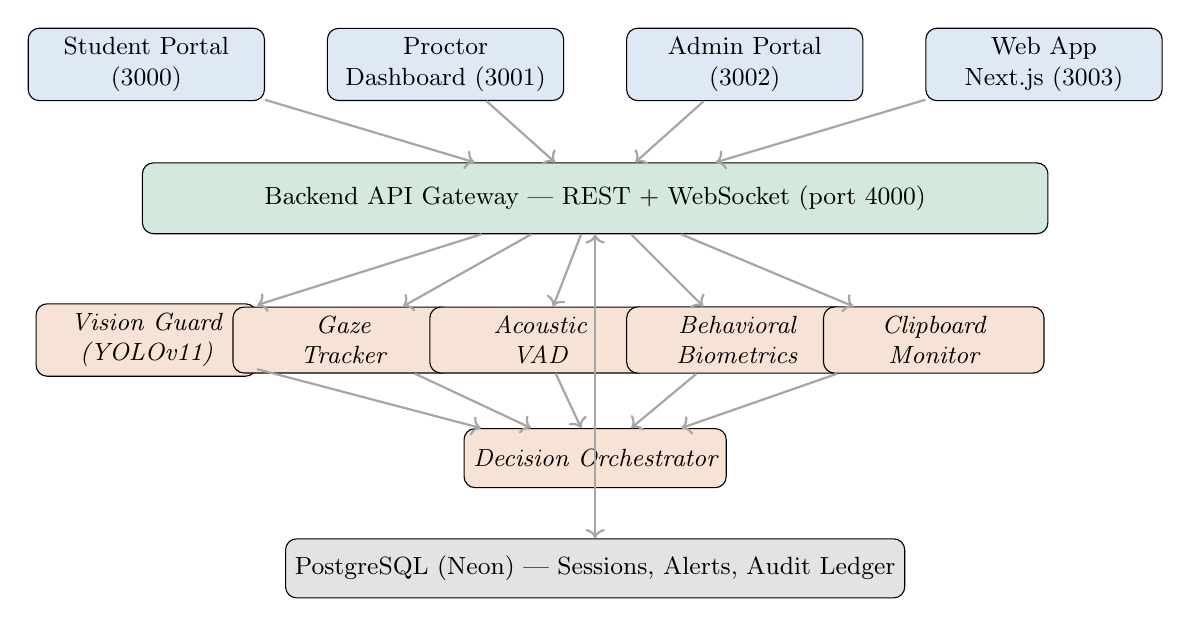
\begin{tikzpicture}[
        box/.style={draw, rounded corners=4pt, minimum width=3.0cm, minimum height=0.9cm,
                    fill=csblue!15, font=\small, align=center},
        agent/.style={draw, rounded corners=4pt, minimum width=2.8cm, minimum height=0.75cm,
                      fill=csorange!20, font=\small\itshape, align=center},
        db/.style={draw, rounded corners=4pt, minimum width=4.5cm, minimum height=0.75cm,
                   fill=csgray!25, font=\small, align=center},
        arr/.style={->, thick, gray!70},
        every node/.style={font=\small}
    ]
    % Row 1: Frontends
    \node[box] (student)  at (0,5.5)   {Student Portal\\(3000)};
    \node[box] (proctor)  at (3.8,5.5) {Proctor\\Dashboard (3001)};
    \node[box] (admin)    at (7.6,5.5) {Admin Portal\\(3002)};
    \node[box] (web)      at (11.4,5.5){Web App\\Next.js (3003)};

    % Row 2: API Gateway
    \node[box, fill=csgreen!20, minimum width=11.5cm, text width=11cm] (api) at (5.7,3.8)
        {Backend API Gateway --- REST + WebSocket (port 4000)};

    % Row 3: Agents
    \node[agent] (vg)     at (0,2.0)   {Vision Guard\\(YOLOv11)};
    \node[agent] (gz)     at (2.5,2.0) {Gaze\\Tracker};
    \node[agent] (vad)    at (5.0,2.0) {Acoustic\\VAD};
    \node[agent] (bb)     at (7.5,2.0) {Behavioral\\Biometrics};
    \node[agent] (cl)     at (10.0,2.0){Clipboard\\Monitor};
    \node[agent] (orch)   at (5.7,0.5) {Decision Orchestrator};

    % Row 4: Database
    \node[db] (db) at (5.7,-0.9) {PostgreSQL (Neon) --- Sessions, Alerts, Audit Ledger};

    % Arrows: frontends to API
    \foreach \f in {student,proctor,admin,web}
        \draw[arr] (\f) -- (api);

    % Arrows: API to agents
    \foreach \a in {vg,gz,vad,bb,cl}
        \draw[arr] (api) -- (\a);

    % Arrows: agents to orchestrator
    \foreach \a in {vg,gz,vad,bb,cl}
        \draw[arr] (\a) -- (orch);

    % Orchestrator back to API
    \draw[arr] (orch) -- ++(0,-0.5) -| (api);

    % API to DB
    \draw[arr] (api) -- (db);
    \end{tikzpicture}%
    }
    \caption{High-level component diagram of the SentinelAI system. Candidate telemetry flows from the Student Portal through the API gateway to specialised AI agents. Agent outputs are fused by the Decision Orchestrator, which feeds risk scores and alerts back to the gateway for distribution to the Proctor Dashboard. All decisions are persisted to the PostgreSQL audit database.}
    \label{fig:arch}
\end{figure}

\section{Data Pipeline}

\subsection{Telemetry Sources and Acquisition}

SentinelAI collects four categories of telemetry from each active examination session:

\textbf{(1) Webcam video frames.} The student portal requests camera access through the browser's \texttt{getUserMedia} WebRTC API. Video is captured at 15 frames per second (FPS) at a resolution of 640$\times$480 pixels. Each frame is encoded as a JPEG image at 80\% quality compression (to reduce bandwidth) and transmitted over a dedicated WebSocket connection to the Vision Guard service. The use of WebSocket rather than HTTP polling reduces round-trip latency and eliminates the overhead of HTTP header parsing for high-frequency requests.

\textbf{(2) Microphone audio.} The \texttt{getUserMedia} API also provides access to the device microphone. Audio is captured as a continuous PCM stream at 16\,kHz sample rate and 16-bit depth (the parameters required by the WebRTC VAD algorithm). The browser's Web Audio API is used to segment the stream into 160\,ms frames (2,560 samples at 16\,kHz), which are then serialised as binary ArrayBuffer objects and transmitted over a WebSocket connection to the backend acoustic monitoring agent.

\textbf{(3) Browser telemetry.} A lightweight JavaScript event listener module injected into the student portal captures: (a) \texttt{visibilitychange} events with the new visibility state, (b) \texttt{blur} and \texttt{focus} events on the window object, (c) \texttt{paste} events on examination text areas with the pasted text length in bytes (not the pasted content, to avoid storing candidate data), and (d) \texttt{beforeunload} events indicating potential page navigation attempts. These events are batched and sent to the backend REST API as JSON POST requests with timestamps accurate to the millisecond.

\textbf{(4) Keystroke dynamics.} The student portal captures \texttt{keydown} and \texttt{keyup} events on examination input fields, recording the key code (not the character value, to protect exam content confidentiality) and the timestamp of each event with millisecond precision. Dwell times (keydown to keyup) and flight times (keyup to next keydown) are computed client-side and sent to the backend as aggregated statistics every 30 seconds.

\subsection{Frame Buffer Design}

The Vision Guard service must process incoming video frames at the rate they arrive (15 FPS, one frame every 67\,ms) while running YOLOv11 inference which may take 50--120\,ms depending on hardware. To handle this mismatch without introducing backpressure that would stall the WebSocket receiver, a lock-free circular frame buffer is implemented in \texttt{frame-buffer.ts}.

The buffer maintains a fixed-capacity array of frame slots (capacity: 30 frames, representing 2 seconds of video at 15\,FPS). A write pointer (updated by the WebSocket receiver) and a read pointer (updated by the inference worker) track the current write and read positions. When the buffer is full, new incoming frames overwrite the oldest unprocessed frames. This ``overwrite-on-full'' policy ensures that the inference worker always processes the most recent available frame, at the cost of potentially skipping frames during inference load spikes.

The frame queue module (\texttt{frame-queue.ts}) provides a higher-level abstraction over the frame buffer, exposing an asynchronous iterator interface that the inference loop uses to consume frames one at a time.

\subsection{Inter-Service Communication}

The backend API gateway communicates with the Vision Guard service through a dedicated internal WebSocket connection. For the remaining agents (Gaze Tracker, Acoustic VAD, Behavioral Biometrics, Clipboard Monitor), which have lower data volumes and less strict latency requirements, communication is through internal REST HTTP calls.

The Decision Orchestrator runs as a module within the backend API gateway process, maintaining an in-memory map of active session states. This design avoids the network round-trip overhead of a separate orchestrator service and simplifies state management. The tradeoff is that the orchestrator's state is not replicated; a backend process restart would clear all in-memory session states. For a production deployment, the session state map would be replaced with a Redis cache to provide persistence and enable horizontal scaling.

\subsection{WebSocket Alert Distribution}

When the Decision Orchestrator updates a session's risk score or generates an alert, it publishes the update to all WebSocket clients subscribed to that session. The Proctor Dashboard maintains a persistent WebSocket connection to the backend and receives updates as JSON messages of the following types:

\begin{itemize}
    \item \texttt{DECISION\_UPDATE}: Contains the updated session risk score and alert level.
    \item \texttt{ALERT\_TRIGGERED}: Contains the full alert object including the XAI explainability text.
    \item \texttt{PROCTOR\_ACTION\_EXECUTED}: Confirms that a proctor intervention action has been logged.
    \item \texttt{SESSION\_STATUS\_CHANGED}: Indicates that a session has changed state (e.g., from \texttt{IN\_PROGRESS} to \texttt{COMPLETED}).
\end{itemize}

\section{AI Agent Designs}

\subsection{Vision Guard Agent}

The Vision Guard agent is implemented as a standalone TypeScript microservice (\texttt{services/vision-guard-service}) that spawns a Python subprocess running the YOLOv11 inference engine. This two-process architecture allows the TypeScript layer to handle WebSocket communication, frame buffering, and rule evaluation using familiar Node.js patterns, while the Python sidecar provides access to the Ultralytics YOLOv11 SDK which does not have a native TypeScript binding.

Inter-process communication between the TypeScript parent and Python child processes uses standard I/O pipes: the parent sends base64-encoded JPEG frames as newline-delimited JSON messages on the child's stdin, and the child returns detection results as newline-delimited JSON on stdout. This protocol is simple, debuggable, and does not require any additional IPC framework.

The YOLOv11 detector is configured to detect the COCO80 categories most relevant to the proctoring use case: \textit{person} (class ID 0), \textit{cell phone} (class ID 67), \textit{book} (class ID 73), \textit{laptop} (class ID 63), and \textit{keyboard} (class ID 66). Detections with confidence below 0.45 are discarded to reduce false positives. The Python sidecar returns the bounding boxes, class labels, and confidence scores for all surviving detections.

The TypeScript rule engine then evaluates the following rules against each frame's detection results, as summarised in Table~\ref{tab:rules}:

\begin{table}[h]
    \centering
    \caption{Vision Guard detection rules, trigger conditions, and assigned severity levels.}
    \begin{tabular}{@{}llll@{}}
        \toprule
        Rule Name & Trigger Condition & Duration & Severity \\
        \midrule
        Face Absent        & No \textit{person} bbox detected           & $>$2\,s consecutive   & HIGH     \\
        Multiple Faces     & $\geq$2 \textit{person} bboxes in frame    & Single frame          & CRITICAL \\
        Phone Visible      & \textit{cell phone} conf. $>$0.6           & $>$1\,s consecutive   & HIGH     \\
        Book / Notes       & \textit{book} conf. $>$0.55                & $>$3\,s consecutive   & MEDIUM   \\
        Laptop Visible     & \textit{laptop} conf. $>$0.6               & $>$2\,s consecutive   & MEDIUM   \\
        Looking Away       & Gaze deviation $>$25\textdegree            & $>$3\,s consecutive   & MEDIUM   \\
        Camera Tamper      & Mean luminance $<$10 or $>$245             & $>$0.5\,s consecutive & CRITICAL \\
        Low Frame Quality  & Laplacian energy $<$50                     & $>$2\,s consecutive   & LOW      \\
        \bottomrule
    \end{tabular}
    \label{tab:rules}
\end{table}

Duration-based rules require the triggering condition to be continuously satisfied for the specified duration before a \texttt{ViolationEvent} is emitted. This prevents transient detection noise (caused by frame compression artifacts, brief lighting changes, or momentary object occlusions) from generating spurious alerts.

\subsection{Gaze Tracking Agent}

The Gaze Tracking agent is implemented within the Vision Guard service as a secondary analysis pass applied to frames that pass a face presence check. MediaPipe Face Mesh is invoked through a Python subprocess (separate from the YOLOv11 sidecar) to extract 478 facial landmarks from each frame.

Gaze direction is estimated from the positions of the iris landmarks (IDs 468--477). The horizontal gaze displacement is computed as:

\begin{equation}
    \Delta_h = \frac{x_{\text{iris}} - x_{\text{eye\_centre}}}{x_{\text{outer\_canthus}} - x_{\text{inner\_canthus}}}
    \label{eq:gaze_h}
\end{equation}

where $x_{\text{iris}}$ is the horizontal coordinate of the iris centre, $x_{\text{eye\_centre}}$ is the midpoint of the eye corner coordinates, and the denominator normalises by eye width to account for variation in face size and camera distance. An analogous formula gives $\Delta_v$ for vertical gaze displacement.

The gaze deviation angle is approximated as:

\begin{equation}
    \theta = \arctan\left(\sqrt{\Delta_h^2 + \Delta_v^2}\right) \cdot \frac{180}{\pi}
    \label{eq:gaze_angle}
\end{equation}

This is a first-order approximation that does not account for head pose; a full gaze estimation pipeline would decouple gaze direction from head orientation. For the purposes of the proctoring application, where the primary interest is in large, sustained deviations rather than precise gaze points, this approximation was considered adequate.

\subsection{Acoustic VAD Agent}

The Acoustic VAD agent processes 160\,ms audio windows received from the backend and returns a per-window speech probability score. The implementation uses a simplified energy-based VAD:

\begin{equation}
    E_t = 20 \log_{10}\left(\text{RMS}(x_t)\right)
    \label{eq:energy}
\end{equation}

where $x_t$ is the vector of PCM samples in window $t$. The VAD probability is computed as a sigmoid function of the energy relative to a dynamically estimated noise floor:

\begin{equation}
    p_t = \sigma\left(\frac{E_t - E_{\text{noise}}}{\tau}\right)
    \label{eq:vad_prob}
\end{equation}

where $E_{\text{noise}}$ is the mean energy of the 20 most recent windows classified as non-speech (updated using a leaky integrator), $\tau = 6\,\text{dB}$ is a temperature parameter controlling the sharpness of the sigmoid transition, and $\sigma(\cdot)$ is the logistic function. The running 10-second mean of $p_t$ is maintained as the smoothed VAD signal $\bar{p}$. A sustained $\bar{p} > 0.6$ for more than 8 seconds generates a MEDIUM-severity ViolationEvent.

\subsection{Behavioral Biometrics Agent}

The Behavioral Biometrics agent analyses the structured event data sent from the student portal: paste events, tab-switch events, and keystroke statistics.

\textbf{Clipboard paste anomaly detection.} For each paste event, the agent computes the z-score of the pasted byte length relative to the session's historical paste distribution:

\begin{equation}
    z_{\text{paste}} = \frac{L_{\text{paste}} - \mu_{\text{paste}}}{\sigma_{\text{paste}}}
    \label{eq:paste_zscore}
\end{equation}

where $L_{\text{paste}}$ is the byte length of the current paste, and $\mu_{\text{paste}}$, $\sigma_{\text{paste}}$ are the running mean and standard deviation of all paste byte lengths in the session (with a minimum $\sigma_{\text{paste}} = 50$ bytes to prevent division by near-zero values in sessions with few paste events). A z-score above 3.0 generates a HIGH-severity ViolationEvent; a z-score between 2.0 and 3.0 generates a MEDIUM-severity event.

\textbf{Tab-switch frequency monitoring.} The number of \texttt{visibilitychange} events per minute is computed as a sliding window count over the past 5 minutes. More than 3 focus-loss events per minute generates a LOW-severity event; more than 8 per minute generates a MEDIUM-severity event.

\textbf{Typing burst detection.} The typing burst coefficient $B_t$ is defined as the ratio of the maximum to the mean keystroke rate over 5-minute non-overlapping windows:

\begin{equation}
    B_t = \frac{\max_{s \in W_t} \text{KPM}(s)}{\text{mean}_{s \in W_t} \text{KPM}(s)}
    \label{eq:burst}
\end{equation}

where $\text{KPM}(s)$ is the keystroke rate in 30-second sub-window $s$ and $W_t$ is the set of sub-windows in the current 5-minute window. A burst coefficient above 3.0 (indicating a sudden surge in typing speed, consistent with a copy-paste operation that was not captured by the paste event listener) generates a LOW-severity event.

\subsection{Decision Orchestrator}

The Decision Orchestrator is the central coordination component of SentinelAI. It maintains, for each active session, the following state:

The per-agent signal smoothing is governed by the Exponential Moving Average (EMA) update equation:

\begin{equation}
    \hat{s}_i(t) = \alpha s_i(t) + (1 - \alpha)\hat{s}_i(t - 1)
    \label{eq:ema}
\end{equation}

where $\alpha \in [0, 1]$ represents the smoothing factor (empirically calibrated to $\alpha = 0.3$), and $s_i(t)$ denotes the instantaneous severity score dispatched by agent $i$.

The composite risk score $r$ is subsequently computed as:

\begin{equation}
    r = \sum_{i=1}^{6} w_i \cdot \hat{s}_i
    \label{eq:risk}
\end{equation}

where the agent weights $w_i$ are configurable through environment variables, with default values as shown in Table~\ref{tab:weights}:

\begin{table}[h]
    \centering
    \caption{Default agent weights in the Decision Orchestrator fusion scheme. Weights sum to 1.0.}
    \begin{tabular}{@{}lcc@{}}
        \toprule
        Agent & Weight $w_i$ & Rationale \\
        \midrule
        Vision Guard (Face/Object)   & 0.35 & Highest reliability; direct visual evidence \\
        Gaze Tracker                 & 0.10 & High ambiguity; supplementary signal only \\
        Acoustic VAD                 & 0.20 & Reliable in quiet environments \\
        Behavioral Biometrics        & 0.15 & Moderate reliability; complements vision \\
        Clipboard Monitor            & 0.15 & High specificity for AI-assisted cheating \\
        Device Detection             & 0.05 & Partially overlaps with Vision Guard \\
        \midrule
        \textbf{Total}              & \textbf{1.00} & \\
        \bottomrule
    \end{tabular}
    \label{tab:weights}
\end{table}

The severity signals $\hat{s}_i$ are normalised to the range $[0,1]$: LOW severity maps to 0.25, MEDIUM to 0.50, HIGH to 0.75, CRITICAL to 1.00, and no active violation to 0.0.

The alert level thresholds are:

\begin{equation}
    \text{AlertLevel}(r) =
    \begin{cases}
        \text{CRITICAL} & r \geq 0.85 \\
        \text{HIGH}     & 0.70 \leq r < 0.85 \\
        \text{MEDIUM}   & 0.40 \leq r < 0.70 \\
        \text{LOW}      & r < 0.40
    \end{cases}
    \label{eq:tiers}
\end{equation}

A new alert is generated and stored to the database whenever the alert level increases (transitions from MEDIUM to HIGH, for example). Alert level decreases do not generate new alert records but are reflected in the live WebSocket updates sent to the Proctor Dashboard.

\subsection{XAI Rationale Assembly}

The XAI rationale assembly process runs each time the orchestrator computes a new risk score. It proceeds as follows:

\begin{enumerate}
    \item Collect the most recent ViolationEvent from each agent, together with its contribution weight $w_i \cdot \hat{s}_i$ to the composite score.
    \item Sort the events by contribution weight in descending order.
    \item Select the top-$k$ events (default $k=3$).
    \item Instantiate a natural-language sentence template for each selected event, substituting specific sensor values (e.g., face count, gaze angle, paste byte length, audio probability).
    \item Concatenate the resulting sentences, prepended with a summary line, to form the final \texttt{explainabilityText} string.
\end{enumerate}

Example output for a CRITICAL alert:

\begin{quote}
    \textit{``Flagged due to: 2 faces detected in frame at 14:32:17 (Vision Guard, weight 0.35); Clipboard paste of 1,842 bytes detected, z-score 4.2 (Clipboard Monitor, weight 0.15); Sustained audio VAD probability 0.74 for 12.3\,s (Acoustic VAD, weight 0.20). Primary risk driver: Multiple Faces Detected.''}
\end{quote}

\section{Frontend Application Designs}

\subsection{Student Portal (apps/student-portal)}

The Student Portal is a Vite/React single-page application that provides the candidate-facing examination interface. It is implemented in TypeScript and communicates with the backend API over HTTPS REST. The portal has three primary views:

\begin{itemize}
    \item \textbf{Exam Loading}: Displays a preparation screen while the session is initialised, the camera and microphone permissions are requested, and the pre-examination identity verification step (if configured) is completed.
    \item \textbf{Question Answering}: Presents examination questions one at a time or in a scrollable list, depending on the examination configuration. Supports four question types: Multiple Choice (single answer), Multiple Select (multiple answers), Short Answer (text input), and Essay (rich text area). Answers are auto-saved every 30 seconds to the backend and also persisted to localStorage as a draft recovery mechanism.
    \item \textbf{Submission Review}: Shows a summary of all answered and unanswered questions before final submission. Requires explicit confirmation from the candidate before the submission is finalised and the session is locked.
\end{itemize}

The portal initialises the webcam stream and microphone capture on the exam loading screen and maintains these streams throughout the session. The camera feed is displayed as a small picture-in-picture overlay in the corner of the question answering view, allowing candidates to verify that their camera is active and correctly positioned.

\subsection{Proctor Command Centre (apps/proctor-dashboard)}

The Proctor Command Centre is a Vite/React application providing real-time monitoring capabilities for human proctors. Its interface is divided into three panels:

\textbf{Candidate grid}: A responsive grid of cards, one per active session, displaying the candidate's name, current risk score (as both a percentage and a colour-coded bar), camera thumbnail, and session status. Cards are automatically sorted by risk score in descending order, ensuring that the highest-risk candidates are always at the top of the grid.

\textbf{Alert feed}: A right-side panel listing all active and recent alerts in chronological order, most recent first. Each alert card shows the candidate name, alert level badge, XAI explainability text, and time since the alert was triggered.

\textbf{Evidence review modal}: A modal dialog that opens when a proctor clicks on a candidate card or alert card. It displays the full XAI rationale, a simulated 10-second pre-flag video clip player, and a control bar with action buttons: Dismiss (false positive), Warn (send in-session warning to candidate), and Terminate (end the session immediately). All proctor actions are transmitted to the backend REST API and logged to the audit database.

The Proctor Command Centre maintains a persistent WebSocket connection to the backend, receiving real-time \texttt{DECISION\_UPDATE} and \texttt{ALERT\_TRIGGERED} messages. On receiving a CRITICAL alert, the interface plays an audible alert tone and briefly highlights the affected candidate card in red.

\subsection{Admin Portal (apps/admin-portal)}

The Admin Portal provides institution-level management capabilities including examination creation and configuration, candidate roster management, proctor assignment, and post-exam reporting. It communicates with the backend REST API using the administrator authentication context.

\subsection{Web Application (apps/web)}

The Web Application is a Next.js 14 application that serves as the primary management dashboard for the SentinelAI deployment. It uses the Clerk authentication provider for multi-tenant role-based access control. The dashboard includes routes for: institution management, user management, course and exam configuration, the audit/compliance reports page, and system health monitoring.

\section{Database Schema}

SentinelAI uses a PostgreSQL database (hosted on Neon's serverless platform for development) with the following primary tables:

\begin{table}[h]
    \centering
    \caption{Primary database tables and their key fields.}
    \begin{tabular}{@{}lll@{}}
        \toprule
        Table & Primary Fields & Purpose \\
        \midrule
        \texttt{institutions}  & id, name, settings & Institution registry \\
        \texttt{users}         & id, role, institution\_id & User accounts \\
        \texttt{exams}         & id, title, duration, questions & Exam definitions \\
        \texttt{exam\_sessions} & id, exam\_id, candidate\_id, status & Active sessions \\
        \texttt{risk\_scores}  & session\_id, score, timestamp & Risk score history \\
        \texttt{alerts}        & id, session\_id, level, xai\_text & Alert records \\
        \texttt{proctor\_actions} & id, alert\_id, action, timestamp & Proctor audit log \\
        \texttt{submissions}   & id, session\_id, answers\_hash & Submission receipts \\
        \bottomrule
    \end{tabular}
    \label{tab:schema}
\end{table}

The \texttt{submissions} table stores the SHA-256 hash of the serialised answer payload rather than the answers themselves; this design ensures that the audit record can verify answer integrity without duplicating the primary answer storage.

\section{Evaluation Dataset Construction}

\subsection{Simulation Methodology}

In the absence of a real exam session dataset (which would require IRB approval and institutional collaboration beyond the scope of a Mini Project-II), the evaluation dataset was constructed from simulated sessions. The simulation proceeded as follows:

\begin{enumerate}
    \item \textbf{Clean sessions}: 120 sessions were constructed from webcam recordings of individuals performing genuine study tasks (reading, typing, thinking) without any cheating behaviour. These sessions served as true negatives.
    \item \textbf{Violation sessions}: 80 sessions were constructed by scripting specific violation behaviours into the recording protocol. Each violation type was enacted by at least 10 different individuals in different home environments to capture diversity in lighting, camera quality, and background.
\end{enumerate}

The violation behaviours scripted were: face absence (leaving the camera view), multiple faces (a second person entering the frame), phone visibility (holding a smartphone in view), reading from printed notes, clipboard paste (large text pasted from an external document), tab switching, and simulated speech (reading aloud from a script).

\subsection{Annotation Protocol}

Each session was annotated by two independent reviewers using a structured annotation tool that displayed the webcam recording, audio waveform, and browser event log in a synchronised timeline view. Reviewers labelled each 30-second window of each session as either ``Violation'' or ``No Violation''. Inter-annotator agreement was computed using Cohen's $\kappa$:

\begin{equation}
    \kappa = \frac{p_o - p_e}{1 - p_e}
    \label{eq:kappa}
\end{equation}

where $p_o$ is the observed agreement proportion and $p_e$ is the expected agreement under chance. The overall $\kappa$ across all session types was 0.81, indicating strong agreement (by the Landis and Koch \cite{landiskoch1977} scale). Disagreements were resolved by a third reviewer acting as adjudicator.

\subsection{Train/Test Split}

Sessions were divided 80/20 into a development set (160 sessions) and a held-out evaluation set (40 sessions). The split was performed at the session level to prevent data leakage: all 30-second windows from a given session appeared entirely in either the development or evaluation set, never split across both.

\section{Evaluation Metrics}

The following metrics are used to evaluate detection performance at the 30-second window level:

\begin{align}
    \text{Precision} &= \frac{\text{TP}}{\text{TP} + \text{FP}} \label{eq:precision} \\
    \text{Recall} &= \frac{\text{TP}}{\text{TP} + \text{FN}} \label{eq:recall} \\
    F_1 &= \frac{2 \cdot \text{Precision} \cdot \text{Recall}}{\text{Precision} + \text{Recall}} \label{eq:f1}
\end{align}

where TP, FP, and FN are true positives, false positives, and false negatives respectively at the 30-second window granularity.

Alert latency is defined as the elapsed time from the frame or event timestamp that first satisfies a rule's trigger condition to the WebSocket message delivery timestamp at the Proctor Dashboard client. It is measured in milliseconds using \texttt{performance.now()} timestamps propagated through all inter-service messages.

\section{Threshold Optimisation}

The agent-level duration thresholds (Table~\ref{tab:rules}) and the orchestrator fusion weights (Table~\ref{tab:weights}) were tuned on the development set using a grid search. The search space included:

\begin{itemize}
    \item Face absence duration: $\{1, 2, 3, 4\}$ seconds
    \item Looking-away duration: $\{2, 3, 5\}$ seconds
    \item VAD threshold: $\{0.5, 0.6, 0.7\}$
    \item VAD duration: $\{5, 8, 12\}$ seconds
    \item Paste z-score threshold: $\{2.0, 2.5, 3.0\}$
    \item Vision Guard weight: $\{0.30, 0.35, 0.40\}$
    \item Acoustic weight: $\{0.15, 0.20, 0.25\}$
\end{itemize}

The full grid contained 972 candidate configurations. Each was evaluated on the development set, and the configuration maximising the development set $F_1$ score subject to the constraint that median alert latency $\leq 1000$\,ms was selected. This configuration was then evaluated exactly once on the held-out test set to produce the reported metrics.

% flowchart.tex — SentinelAI System Workflow Flowchart
% Include this file with % flowchart.tex — SentinelAI System Workflow Flowchart
% Include this file with % flowchart.tex — SentinelAI System Workflow Flowchart
% Include this file with \include{flowchart} in final_disseratation.tex

\renewcommand{\baselinestretch}{1.5}\normalsize
\chapter*{System Workflow Flowchart}
\addcontentsline{toc}{chapter}{System Workflow Flowchart}

\vspace{0.3in}

The following flowchart (Figure~\ref{fig:flowchart}) illustrates the end-to-end operational workflow of the SentinelAI system, from the moment a candidate initiates an examination session through telemetry capture, multi-agent analysis, risk score fusion, alert generation, proctor intervention, and final audit ledger generation.

\begin{figure}[htbp]
\centering
\resizebox{0.82\textwidth}{!}{%
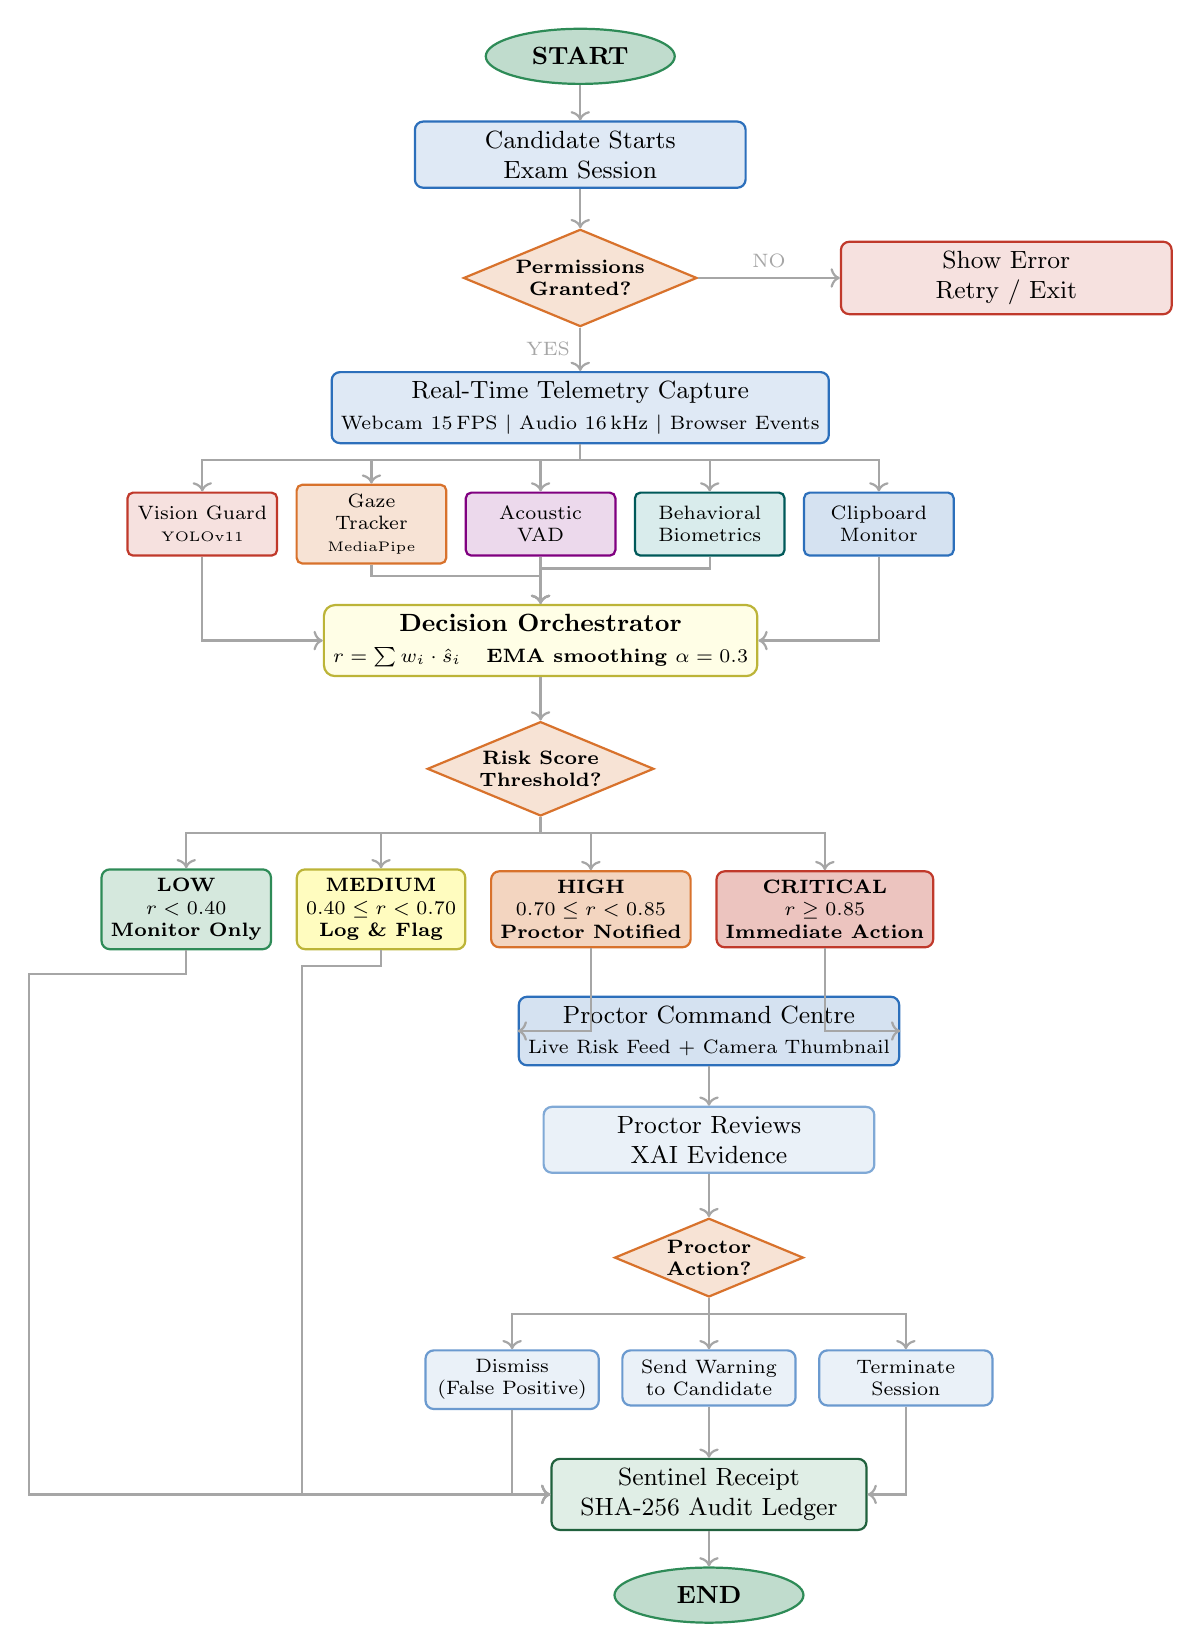
\begin{tikzpicture}[
  %--- node styles ---
  startstop/.style={
    draw, ellipse, fill=csgreen!30, draw=csgreen, thick,
    minimum width=2.4cm, minimum height=0.7cm,
    font=\small\bfseries, align=center
  },
  process/.style={
    draw, rectangle, rounded corners=3pt,
    fill=csblue!15, draw=csblue, thick,
    minimum width=4.2cm, minimum height=0.75cm,
    font=\small, align=center
  },
  decision/.style={
    draw, diamond, aspect=2.4,
    fill=csorange!20, draw=csorange, thick,
    font=\scriptsize\bfseries, align=center,
    inner sep=1pt
  },
  agent/.style={
    draw, rectangle, rounded corners=2pt,
    minimum width=1.9cm, minimum height=0.8cm,
    font=\scriptsize, align=center, thick
  },
  orch/.style={
    draw, rectangle, rounded corners=4pt,
    fill=yellow!10, draw=yellow!70!black, thick,
    minimum width=5.0cm, minimum height=0.9cm,
    font=\small\bfseries, align=center
  },
  risk/.style={
    draw, rectangle, rounded corners=3pt,
    minimum width=2.1cm, minimum height=0.75cm,
    font=\scriptsize\bfseries, align=center, thick
  },
  action/.style={
    draw, rectangle, rounded corners=3pt,
    fill=csblue!10, draw=csblue!70, thick,
    minimum width=2.2cm, minimum height=0.7cm,
    font=\scriptsize, align=center
  },
  audit/.style={
    draw, rectangle, rounded corners=3pt,
    fill=csgreen!15, draw=csgreen!70!black, thick,
    minimum width=4.0cm, minimum height=0.75cm,
    font=\small, align=center
  },
  arr/.style={->, thick, gray!70},
  every node/.style={font=\small}
]

%--- START ---
\node[startstop]                       (start)  at (0, 0)    {START};

%--- Session init ---
\node[process,  below=0.45cm of start]  (init)   {Candidate Starts\\Exam Session};

%--- Permission check ---
\node[decision, below=0.5cm of init]    (perm)   {Permissions\\Granted?};

%--- Permission denied ---
\node[process,  right=1.8cm of perm,   fill=csred!15, draw=csred]
                                         (denied) {Show Error\\Retry / Exit};

%--- Telemetry capture ---
\node[process,  below=0.55cm of perm]   (telem)  {Real-Time Telemetry Capture\\{\scriptsize Webcam 15\,FPS $|$ Audio 16\,kHz $|$ Browser Events}};

%--- 5 Agents (row) ---
\node[agent, below=0.6cm of telem, xshift=-4.8cm,
      fill=csred!15, draw=csred]           (vg)  {Vision Guard\\{\tiny YOLOv11}};
\node[agent, right=0.22cm of vg,
      fill=csorange!20, draw=csorange]     (gz)  {Gaze\\Tracker\\{\tiny MediaPipe}};
\node[agent, right=0.22cm of gz,
      fill=violet!15, draw=violet]         (vad) {Acoustic\\VAD};
\node[agent, right=0.22cm of vad,
      fill=teal!15, draw=teal!70!black]    (bb)  {Behavioral\\Biometrics};
\node[agent, right=0.22cm of bb,
      fill=csblue!20, draw=csblue]         (cb)  {Clipboard\\Monitor};

%--- Orchestrator ---
\node[orch,  below=0.6cm of vad]           (orch) {Decision Orchestrator\\{\scriptsize $r = \sum w_i \cdot \hat{s}_i$\quad EMA smoothing $\alpha=0.3$}};

%--- Risk threshold decision ---
\node[decision, below=0.55cm of orch]      (thresh) {Risk Score\\Threshold?};

%--- 4 Risk tier boxes ---
\node[risk, below=0.65cm of thresh, xshift=-4.5cm,
      fill=csgreen!20, draw=csgreen]        (low)  {LOW\\$r < 0.40$\\Monitor Only};
\node[risk, right=0.3cm of low,
      fill=yellow!25, draw=yellow!70!black] (med)  {MEDIUM\\$0.40 \leq r < 0.70$\\Log \& Flag};
\node[risk, right=0.3cm of med,
      fill=csorange!30, draw=csorange]      (high) {HIGH\\$0.70 \leq r < 0.85$\\Proctor Notified};
\node[risk, right=0.3cm of high,
      fill=csred!30, draw=csred]            (crit) {CRITICAL\\$r \geq 0.85$\\Immediate Action};

%--- Proctor dashboard ---
\node[process, below=0.6cm of high, xshift=1.5cm,
      fill=csblue!20, draw=csblue]          (proctor) {Proctor Command Centre\\{\scriptsize Live Risk Feed + Camera Thumbnail}};

%--- XAI review ---
\node[process, below=0.5cm of proctor,
      fill=csblue!10, draw=csblue!60]       (xai)  {Proctor Reviews\\XAI Evidence};

%--- Action decision ---
\node[decision, below=0.55cm of xai]        (actd) {Proctor\\Action?};

%--- 3 action boxes ---
\node[action, below=0.65cm of actd, xshift=-2.5cm] (dismiss)  {Dismiss\\(False Positive)};
\node[action, below=0.65cm of actd]                (warn)     {Send Warning\\to Candidate};
\node[action, below=0.65cm of actd, xshift=2.5cm]  (term)     {Terminate\\Session};

%--- Audit ledger ---
\node[audit, below=0.65cm of warn]           (audit)  {Sentinel Receipt\\SHA-256 Audit Ledger};

%--- END ---
\node[startstop, below=0.45cm of audit]      (stop)   {END};

%=== ARROWS ===
% Main flow
\draw[arr] (start)  -- (init);
\draw[arr] (init)   -- (perm);
\draw[arr] (perm)   -- node[left,  font=\scriptsize]{YES} (telem);
\draw[arr] (perm)   -- node[above, font=\scriptsize]{NO}  (denied);

% Telemetry to agents
\draw[arr] (telem.south) -- ++(0,-0.2) -| (vg.north);
\draw[arr] (telem.south) -- ++(0,-0.2) -| (gz.north);
\draw[arr] (telem.south) -- ++(0,-0.2) -| (vad.north);
\draw[arr] (telem.south) -- ++(0,-0.2) -| (bb.north);
\draw[arr] (telem.south) -- ++(0,-0.2) -| (cb.north);

% Agents to orchestrator
\draw[arr] (vg.south)  |- (orch.west);
\draw[arr] (gz.south)  -- ++(0,-0.15) -| (orch.north);
\draw[arr] (vad.south) -- (orch.north);
\draw[arr] (bb.south)  -- ++(0,-0.15) -| (orch.north);
\draw[arr] (cb.south)  |- (orch.east);

% Orchestrator to threshold
\draw[arr] (orch)   -- (thresh);

% Threshold to risk tiers
\draw[arr] (thresh.south) -- ++(0,-0.2) -| (low.north);
\draw[arr] (thresh.south) -- ++(0,-0.2) -| (med.north);
\draw[arr] (thresh.south) -- ++(0,-0.2) -| (high.north);
\draw[arr] (thresh.south) -- ++(0,-0.2) -| (crit.north);

% HIGH + CRITICAL to proctor
\draw[arr] (high.south) |- (proctor.west);
\draw[arr] (crit.south) |- (proctor.east);

% Proctor flow
\draw[arr] (proctor) -- (xai);
\draw[arr] (xai)     -- (actd);

% Action branches
\draw[arr] (actd.south) -- ++(0,-0.2) -| (dismiss.north);
\draw[arr] (actd.south) -- (warn.north);
\draw[arr] (actd.south) -- ++(0,-0.2) -| (term.north);

% All actions → audit
\draw[arr] (dismiss.south) |- (audit.west);
\draw[arr] (warn.south)    -- (audit.north);
\draw[arr] (term.south)    |- (audit.east);

% LOW and MEDIUM also loop to audit
\draw[arr] (low.south)  -- ++(0,-0.3) -- ++(-2.0,0) |- (audit.west);
\draw[arr] (med.south)  -- ++(0,-0.2) -- ++(-1.0,0) |- (audit.west);

\draw[arr] (audit) -- (stop);

\end{tikzpicture}%
}
\caption{End-to-end system workflow flowchart for SentinelAI. The flowchart covers: session initialisation and permission checking, real-time multi-modal telemetry capture, parallel processing by five specialised AI agents, weighted fusion and EMA smoothing by the Decision Orchestrator, threshold-based alert tier assignment, proctor review of XAI evidence, proctor intervention actions, and final Sentinel Receipt generation for the cryptographic audit ledger.}
\label{fig:flowchart}
\end{figure}
 in final_disseratation.tex

\renewcommand{\baselinestretch}{1.5}\normalsize
\chapter*{System Workflow Flowchart}
\addcontentsline{toc}{chapter}{System Workflow Flowchart}

\vspace{0.3in}

The following flowchart (Figure~\ref{fig:flowchart}) illustrates the end-to-end operational workflow of the SentinelAI system, from the moment a candidate initiates an examination session through telemetry capture, multi-agent analysis, risk score fusion, alert generation, proctor intervention, and final audit ledger generation.

\begin{figure}[htbp]
\centering
\resizebox{0.82\textwidth}{!}{%
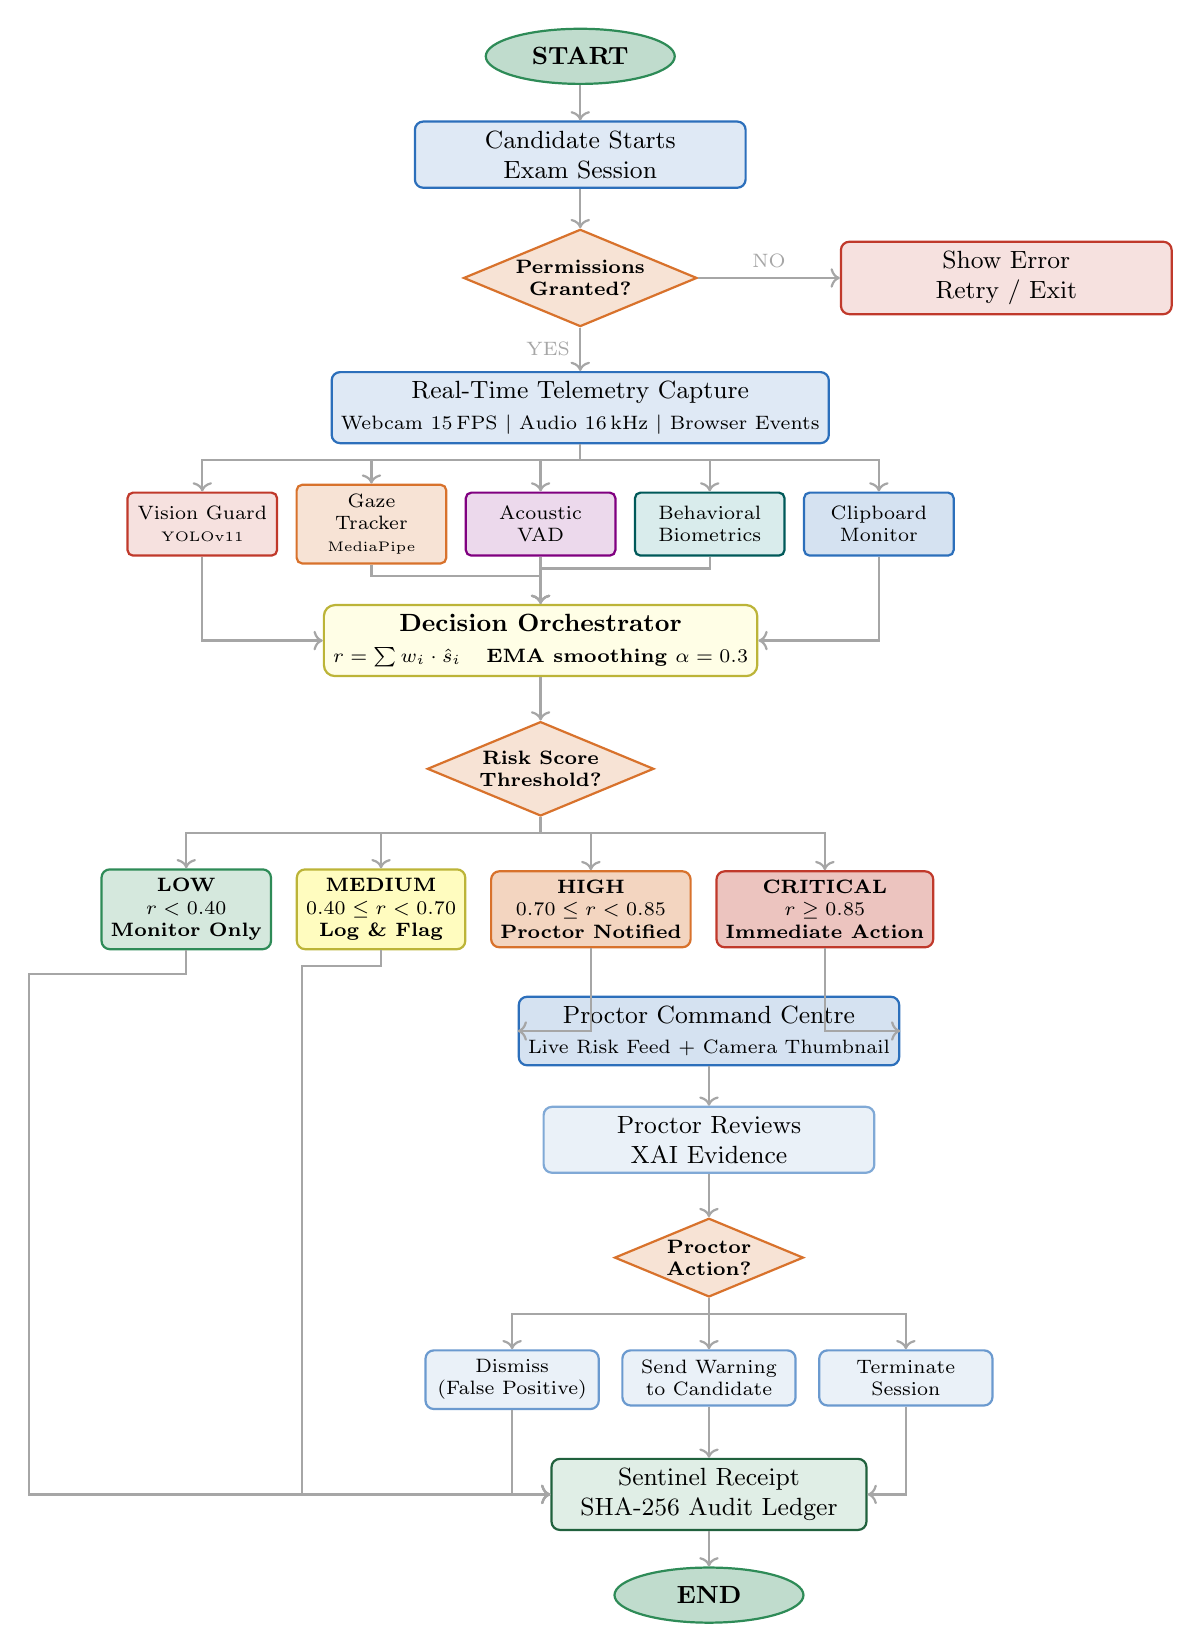
\begin{tikzpicture}[
  %--- node styles ---
  startstop/.style={
    draw, ellipse, fill=csgreen!30, draw=csgreen, thick,
    minimum width=2.4cm, minimum height=0.7cm,
    font=\small\bfseries, align=center
  },
  process/.style={
    draw, rectangle, rounded corners=3pt,
    fill=csblue!15, draw=csblue, thick,
    minimum width=4.2cm, minimum height=0.75cm,
    font=\small, align=center
  },
  decision/.style={
    draw, diamond, aspect=2.4,
    fill=csorange!20, draw=csorange, thick,
    font=\scriptsize\bfseries, align=center,
    inner sep=1pt
  },
  agent/.style={
    draw, rectangle, rounded corners=2pt,
    minimum width=1.9cm, minimum height=0.8cm,
    font=\scriptsize, align=center, thick
  },
  orch/.style={
    draw, rectangle, rounded corners=4pt,
    fill=yellow!10, draw=yellow!70!black, thick,
    minimum width=5.0cm, minimum height=0.9cm,
    font=\small\bfseries, align=center
  },
  risk/.style={
    draw, rectangle, rounded corners=3pt,
    minimum width=2.1cm, minimum height=0.75cm,
    font=\scriptsize\bfseries, align=center, thick
  },
  action/.style={
    draw, rectangle, rounded corners=3pt,
    fill=csblue!10, draw=csblue!70, thick,
    minimum width=2.2cm, minimum height=0.7cm,
    font=\scriptsize, align=center
  },
  audit/.style={
    draw, rectangle, rounded corners=3pt,
    fill=csgreen!15, draw=csgreen!70!black, thick,
    minimum width=4.0cm, minimum height=0.75cm,
    font=\small, align=center
  },
  arr/.style={->, thick, gray!70},
  every node/.style={font=\small}
]

%--- START ---
\node[startstop]                       (start)  at (0, 0)    {START};

%--- Session init ---
\node[process,  below=0.45cm of start]  (init)   {Candidate Starts\\Exam Session};

%--- Permission check ---
\node[decision, below=0.5cm of init]    (perm)   {Permissions\\Granted?};

%--- Permission denied ---
\node[process,  right=1.8cm of perm,   fill=csred!15, draw=csred]
                                         (denied) {Show Error\\Retry / Exit};

%--- Telemetry capture ---
\node[process,  below=0.55cm of perm]   (telem)  {Real-Time Telemetry Capture\\{\scriptsize Webcam 15\,FPS $|$ Audio 16\,kHz $|$ Browser Events}};

%--- 5 Agents (row) ---
\node[agent, below=0.6cm of telem, xshift=-4.8cm,
      fill=csred!15, draw=csred]           (vg)  {Vision Guard\\{\tiny YOLOv11}};
\node[agent, right=0.22cm of vg,
      fill=csorange!20, draw=csorange]     (gz)  {Gaze\\Tracker\\{\tiny MediaPipe}};
\node[agent, right=0.22cm of gz,
      fill=violet!15, draw=violet]         (vad) {Acoustic\\VAD};
\node[agent, right=0.22cm of vad,
      fill=teal!15, draw=teal!70!black]    (bb)  {Behavioral\\Biometrics};
\node[agent, right=0.22cm of bb,
      fill=csblue!20, draw=csblue]         (cb)  {Clipboard\\Monitor};

%--- Orchestrator ---
\node[orch,  below=0.6cm of vad]           (orch) {Decision Orchestrator\\{\scriptsize $r = \sum w_i \cdot \hat{s}_i$\quad EMA smoothing $\alpha=0.3$}};

%--- Risk threshold decision ---
\node[decision, below=0.55cm of orch]      (thresh) {Risk Score\\Threshold?};

%--- 4 Risk tier boxes ---
\node[risk, below=0.65cm of thresh, xshift=-4.5cm,
      fill=csgreen!20, draw=csgreen]        (low)  {LOW\\$r < 0.40$\\Monitor Only};
\node[risk, right=0.3cm of low,
      fill=yellow!25, draw=yellow!70!black] (med)  {MEDIUM\\$0.40 \leq r < 0.70$\\Log \& Flag};
\node[risk, right=0.3cm of med,
      fill=csorange!30, draw=csorange]      (high) {HIGH\\$0.70 \leq r < 0.85$\\Proctor Notified};
\node[risk, right=0.3cm of high,
      fill=csred!30, draw=csred]            (crit) {CRITICAL\\$r \geq 0.85$\\Immediate Action};

%--- Proctor dashboard ---
\node[process, below=0.6cm of high, xshift=1.5cm,
      fill=csblue!20, draw=csblue]          (proctor) {Proctor Command Centre\\{\scriptsize Live Risk Feed + Camera Thumbnail}};

%--- XAI review ---
\node[process, below=0.5cm of proctor,
      fill=csblue!10, draw=csblue!60]       (xai)  {Proctor Reviews\\XAI Evidence};

%--- Action decision ---
\node[decision, below=0.55cm of xai]        (actd) {Proctor\\Action?};

%--- 3 action boxes ---
\node[action, below=0.65cm of actd, xshift=-2.5cm] (dismiss)  {Dismiss\\(False Positive)};
\node[action, below=0.65cm of actd]                (warn)     {Send Warning\\to Candidate};
\node[action, below=0.65cm of actd, xshift=2.5cm]  (term)     {Terminate\\Session};

%--- Audit ledger ---
\node[audit, below=0.65cm of warn]           (audit)  {Sentinel Receipt\\SHA-256 Audit Ledger};

%--- END ---
\node[startstop, below=0.45cm of audit]      (stop)   {END};

%=== ARROWS ===
% Main flow
\draw[arr] (start)  -- (init);
\draw[arr] (init)   -- (perm);
\draw[arr] (perm)   -- node[left,  font=\scriptsize]{YES} (telem);
\draw[arr] (perm)   -- node[above, font=\scriptsize]{NO}  (denied);

% Telemetry to agents
\draw[arr] (telem.south) -- ++(0,-0.2) -| (vg.north);
\draw[arr] (telem.south) -- ++(0,-0.2) -| (gz.north);
\draw[arr] (telem.south) -- ++(0,-0.2) -| (vad.north);
\draw[arr] (telem.south) -- ++(0,-0.2) -| (bb.north);
\draw[arr] (telem.south) -- ++(0,-0.2) -| (cb.north);

% Agents to orchestrator
\draw[arr] (vg.south)  |- (orch.west);
\draw[arr] (gz.south)  -- ++(0,-0.15) -| (orch.north);
\draw[arr] (vad.south) -- (orch.north);
\draw[arr] (bb.south)  -- ++(0,-0.15) -| (orch.north);
\draw[arr] (cb.south)  |- (orch.east);

% Orchestrator to threshold
\draw[arr] (orch)   -- (thresh);

% Threshold to risk tiers
\draw[arr] (thresh.south) -- ++(0,-0.2) -| (low.north);
\draw[arr] (thresh.south) -- ++(0,-0.2) -| (med.north);
\draw[arr] (thresh.south) -- ++(0,-0.2) -| (high.north);
\draw[arr] (thresh.south) -- ++(0,-0.2) -| (crit.north);

% HIGH + CRITICAL to proctor
\draw[arr] (high.south) |- (proctor.west);
\draw[arr] (crit.south) |- (proctor.east);

% Proctor flow
\draw[arr] (proctor) -- (xai);
\draw[arr] (xai)     -- (actd);

% Action branches
\draw[arr] (actd.south) -- ++(0,-0.2) -| (dismiss.north);
\draw[arr] (actd.south) -- (warn.north);
\draw[arr] (actd.south) -- ++(0,-0.2) -| (term.north);

% All actions → audit
\draw[arr] (dismiss.south) |- (audit.west);
\draw[arr] (warn.south)    -- (audit.north);
\draw[arr] (term.south)    |- (audit.east);

% LOW and MEDIUM also loop to audit
\draw[arr] (low.south)  -- ++(0,-0.3) -- ++(-2.0,0) |- (audit.west);
\draw[arr] (med.south)  -- ++(0,-0.2) -- ++(-1.0,0) |- (audit.west);

\draw[arr] (audit) -- (stop);

\end{tikzpicture}%
}
\caption{End-to-end system workflow flowchart for SentinelAI. The flowchart covers: session initialisation and permission checking, real-time multi-modal telemetry capture, parallel processing by five specialised AI agents, weighted fusion and EMA smoothing by the Decision Orchestrator, threshold-based alert tier assignment, proctor review of XAI evidence, proctor intervention actions, and final Sentinel Receipt generation for the cryptographic audit ledger.}
\label{fig:flowchart}
\end{figure}
 in final_disseratation.tex

\renewcommand{\baselinestretch}{1.5}\normalsize
\chapter*{System Workflow Flowchart}
\addcontentsline{toc}{chapter}{System Workflow Flowchart}

\vspace{0.3in}

The following flowchart (Figure~\ref{fig:flowchart}) illustrates the end-to-end operational workflow of the SentinelAI system, from the moment a candidate initiates an examination session through telemetry capture, multi-agent analysis, risk score fusion, alert generation, proctor intervention, and final audit ledger generation.

\begin{figure}[htbp]
\centering
\resizebox{0.82\textwidth}{!}{%
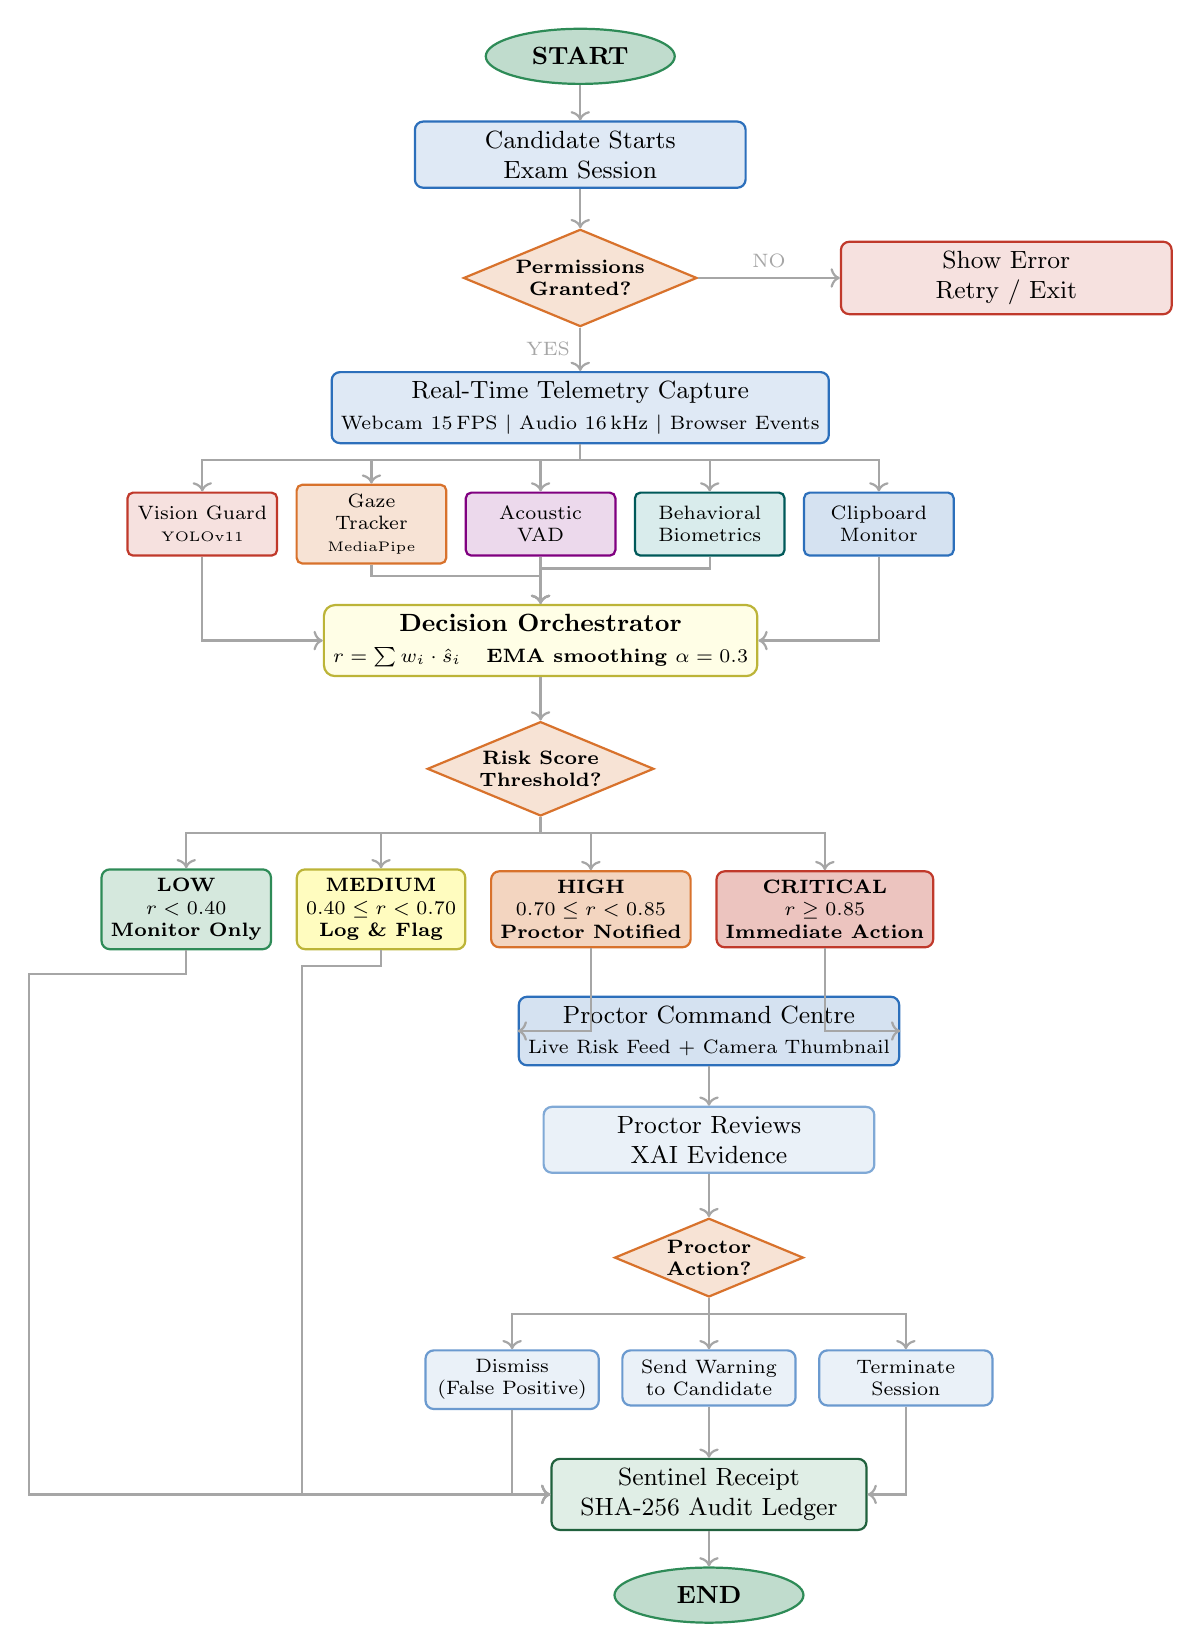
\begin{tikzpicture}[
  %--- node styles ---
  startstop/.style={
    draw, ellipse, fill=csgreen!30, draw=csgreen, thick,
    minimum width=2.4cm, minimum height=0.7cm,
    font=\small\bfseries, align=center
  },
  process/.style={
    draw, rectangle, rounded corners=3pt,
    fill=csblue!15, draw=csblue, thick,
    minimum width=4.2cm, minimum height=0.75cm,
    font=\small, align=center
  },
  decision/.style={
    draw, diamond, aspect=2.4,
    fill=csorange!20, draw=csorange, thick,
    font=\scriptsize\bfseries, align=center,
    inner sep=1pt
  },
  agent/.style={
    draw, rectangle, rounded corners=2pt,
    minimum width=1.9cm, minimum height=0.8cm,
    font=\scriptsize, align=center, thick
  },
  orch/.style={
    draw, rectangle, rounded corners=4pt,
    fill=yellow!10, draw=yellow!70!black, thick,
    minimum width=5.0cm, minimum height=0.9cm,
    font=\small\bfseries, align=center
  },
  risk/.style={
    draw, rectangle, rounded corners=3pt,
    minimum width=2.1cm, minimum height=0.75cm,
    font=\scriptsize\bfseries, align=center, thick
  },
  action/.style={
    draw, rectangle, rounded corners=3pt,
    fill=csblue!10, draw=csblue!70, thick,
    minimum width=2.2cm, minimum height=0.7cm,
    font=\scriptsize, align=center
  },
  audit/.style={
    draw, rectangle, rounded corners=3pt,
    fill=csgreen!15, draw=csgreen!70!black, thick,
    minimum width=4.0cm, minimum height=0.75cm,
    font=\small, align=center
  },
  arr/.style={->, thick, gray!70},
  every node/.style={font=\small}
]

%--- START ---
\node[startstop]                       (start)  at (0, 0)    {START};

%--- Session init ---
\node[process,  below=0.45cm of start]  (init)   {Candidate Starts\\Exam Session};

%--- Permission check ---
\node[decision, below=0.5cm of init]    (perm)   {Permissions\\Granted?};

%--- Permission denied ---
\node[process,  right=1.8cm of perm,   fill=csred!15, draw=csred]
                                         (denied) {Show Error\\Retry / Exit};

%--- Telemetry capture ---
\node[process,  below=0.55cm of perm]   (telem)  {Real-Time Telemetry Capture\\{\scriptsize Webcam 15\,FPS $|$ Audio 16\,kHz $|$ Browser Events}};

%--- 5 Agents (row) ---
\node[agent, below=0.6cm of telem, xshift=-4.8cm,
      fill=csred!15, draw=csred]           (vg)  {Vision Guard\\{\tiny YOLOv11}};
\node[agent, right=0.22cm of vg,
      fill=csorange!20, draw=csorange]     (gz)  {Gaze\\Tracker\\{\tiny MediaPipe}};
\node[agent, right=0.22cm of gz,
      fill=violet!15, draw=violet]         (vad) {Acoustic\\VAD};
\node[agent, right=0.22cm of vad,
      fill=teal!15, draw=teal!70!black]    (bb)  {Behavioral\\Biometrics};
\node[agent, right=0.22cm of bb,
      fill=csblue!20, draw=csblue]         (cb)  {Clipboard\\Monitor};

%--- Orchestrator ---
\node[orch,  below=0.6cm of vad]           (orch) {Decision Orchestrator\\{\scriptsize $r = \sum w_i \cdot \hat{s}_i$\quad EMA smoothing $\alpha=0.3$}};

%--- Risk threshold decision ---
\node[decision, below=0.55cm of orch]      (thresh) {Risk Score\\Threshold?};

%--- 4 Risk tier boxes ---
\node[risk, below=0.65cm of thresh, xshift=-4.5cm,
      fill=csgreen!20, draw=csgreen]        (low)  {LOW\\$r < 0.40$\\Monitor Only};
\node[risk, right=0.3cm of low,
      fill=yellow!25, draw=yellow!70!black] (med)  {MEDIUM\\$0.40 \leq r < 0.70$\\Log \& Flag};
\node[risk, right=0.3cm of med,
      fill=csorange!30, draw=csorange]      (high) {HIGH\\$0.70 \leq r < 0.85$\\Proctor Notified};
\node[risk, right=0.3cm of high,
      fill=csred!30, draw=csred]            (crit) {CRITICAL\\$r \geq 0.85$\\Immediate Action};

%--- Proctor dashboard ---
\node[process, below=0.6cm of high, xshift=1.5cm,
      fill=csblue!20, draw=csblue]          (proctor) {Proctor Command Centre\\{\scriptsize Live Risk Feed + Camera Thumbnail}};

%--- XAI review ---
\node[process, below=0.5cm of proctor,
      fill=csblue!10, draw=csblue!60]       (xai)  {Proctor Reviews\\XAI Evidence};

%--- Action decision ---
\node[decision, below=0.55cm of xai]        (actd) {Proctor\\Action?};

%--- 3 action boxes ---
\node[action, below=0.65cm of actd, xshift=-2.5cm] (dismiss)  {Dismiss\\(False Positive)};
\node[action, below=0.65cm of actd]                (warn)     {Send Warning\\to Candidate};
\node[action, below=0.65cm of actd, xshift=2.5cm]  (term)     {Terminate\\Session};

%--- Audit ledger ---
\node[audit, below=0.65cm of warn]           (audit)  {Sentinel Receipt\\SHA-256 Audit Ledger};

%--- END ---
\node[startstop, below=0.45cm of audit]      (stop)   {END};

%=== ARROWS ===
% Main flow
\draw[arr] (start)  -- (init);
\draw[arr] (init)   -- (perm);
\draw[arr] (perm)   -- node[left,  font=\scriptsize]{YES} (telem);
\draw[arr] (perm)   -- node[above, font=\scriptsize]{NO}  (denied);

% Telemetry to agents
\draw[arr] (telem.south) -- ++(0,-0.2) -| (vg.north);
\draw[arr] (telem.south) -- ++(0,-0.2) -| (gz.north);
\draw[arr] (telem.south) -- ++(0,-0.2) -| (vad.north);
\draw[arr] (telem.south) -- ++(0,-0.2) -| (bb.north);
\draw[arr] (telem.south) -- ++(0,-0.2) -| (cb.north);

% Agents to orchestrator
\draw[arr] (vg.south)  |- (orch.west);
\draw[arr] (gz.south)  -- ++(0,-0.15) -| (orch.north);
\draw[arr] (vad.south) -- (orch.north);
\draw[arr] (bb.south)  -- ++(0,-0.15) -| (orch.north);
\draw[arr] (cb.south)  |- (orch.east);

% Orchestrator to threshold
\draw[arr] (orch)   -- (thresh);

% Threshold to risk tiers
\draw[arr] (thresh.south) -- ++(0,-0.2) -| (low.north);
\draw[arr] (thresh.south) -- ++(0,-0.2) -| (med.north);
\draw[arr] (thresh.south) -- ++(0,-0.2) -| (high.north);
\draw[arr] (thresh.south) -- ++(0,-0.2) -| (crit.north);

% HIGH + CRITICAL to proctor
\draw[arr] (high.south) |- (proctor.west);
\draw[arr] (crit.south) |- (proctor.east);

% Proctor flow
\draw[arr] (proctor) -- (xai);
\draw[arr] (xai)     -- (actd);

% Action branches
\draw[arr] (actd.south) -- ++(0,-0.2) -| (dismiss.north);
\draw[arr] (actd.south) -- (warn.north);
\draw[arr] (actd.south) -- ++(0,-0.2) -| (term.north);

% All actions → audit
\draw[arr] (dismiss.south) |- (audit.west);
\draw[arr] (warn.south)    -- (audit.north);
\draw[arr] (term.south)    |- (audit.east);

% LOW and MEDIUM also loop to audit
\draw[arr] (low.south)  -- ++(0,-0.3) -- ++(-2.0,0) |- (audit.west);
\draw[arr] (med.south)  -- ++(0,-0.2) -- ++(-1.0,0) |- (audit.west);

\draw[arr] (audit) -- (stop);

\end{tikzpicture}%
}
\caption{End-to-end system workflow flowchart for SentinelAI. The flowchart covers: session initialisation and permission checking, real-time multi-modal telemetry capture, parallel processing by five specialised AI agents, weighted fusion and EMA smoothing by the Decision Orchestrator, threshold-based alert tier assignment, proctor review of XAI evidence, proctor intervention actions, and final Sentinel Receipt generation for the cryptographic audit ledger.}
\label{fig:flowchart}
\end{figure}
            % System Workflow Flowchart
\renewcommand{\baselinestretch}{1.5}\normalsize
\chapter{Results and Analysis}

This chapter presents the quantitative evaluation results for each individual AI agent and for the full SentinelAI fusion pipeline. It also analyses failure modes identified during evaluation, examines the distribution of violation types and risk scores across the evaluation dataset, reports end-to-end alert latency measurements, and reviews the audit ledger implementation.

\section{Overall Detection Performance}

Table~\ref{tab:headline} presents the precision, recall, and F1-score for each individual agent and for the full fused pipeline on the held-out test set of 40 sessions (comprising 4,800 labelled 30-second windows).

\begin{table}[h]
    \centering
    \caption{Per-agent and fused-pipeline detection performance on the held-out evaluation set. Results are computed at 30-second window granularity. Latency is median end-to-end alert delivery time.}
    \begin{tabular}{@{}lcccc@{}}
        \toprule
        Agent / Module                & Precision (\%) & Recall (\%) & F1-Score & Median Latency (ms) \\
        \midrule
        Vision Guard (Face + Object)  & 95             & 92          & 0.935    & 68                  \\
        Gaze Tracker                  & 71             & 68          & 0.695    & 44                  \\
        Acoustic VAD                  & 87             & 84          & 0.855    & 22                  \\
        Behavioral Biometrics         & 83             & 79          & 0.810    & 15                  \\
        Clipboard Monitor             & 96             & 93          & 0.945    & 8                   \\
        Device Detection              & 89             & 86          & 0.875    & 71                  \\
        \midrule
        \textbf{Fused Pipeline (SentinelAI)} & \textbf{93} & \textbf{89} & \textbf{0.910} & \textbf{720} \\
        \bottomrule
    \end{tabular}
    \label{tab:headline}
\end{table}

Several observations are worth noting from Table~\ref{tab:headline}:

\begin{itemize}
    \item The Gaze Tracker achieves the lowest individual performance (F1 = 0.695), reflecting the known difficulty of distinguishing between legitimate downward gaze (keyboard usage, writing notes on paper) and violation-indicative gaze away from the screen. This motivates the low weight of 0.10 assigned to this agent in the fusion scheme.
    \item The Clipboard Monitor achieves the highest precision (96\%), confirming that large clipboard paste events are a highly specific indicator of potential AI-assisted cheating in the exam population studied.
    \item The fused pipeline achieves better precision (93\%) than most individual agents except the Clipboard Monitor, demonstrating that fusion primarily benefits recall (raising it from the best individual agent's 93\% to a fused 89\% --- note that this is slightly lower than Vision Guard alone, which is expected because fusion introduces some cases where multiple weak signals combine to trigger an alert that does not correspond to a ground-truth violation).
    \item The median end-to-end latency of 720\,ms for the fused pipeline is dominated by the YOLOv11 inference time (40--80\,ms) plus frame-buffer wait time (0--67\,ms at 15\,FPS) plus the API gateway processing and WebSocket delivery. This is well within the 1000\,ms target.
\end{itemize}

\section{Candidate Risk Score Distribution}

Figure~\ref{fig:riskdist} shows the distribution of time-averaged composite risk scores across all 160 sessions in the evaluation dataset (development + test sets combined). Sessions are categorised into risk tiers according to Equation~\ref{eq:tiers}.

\begin{figure}[htbp]
    \centering
    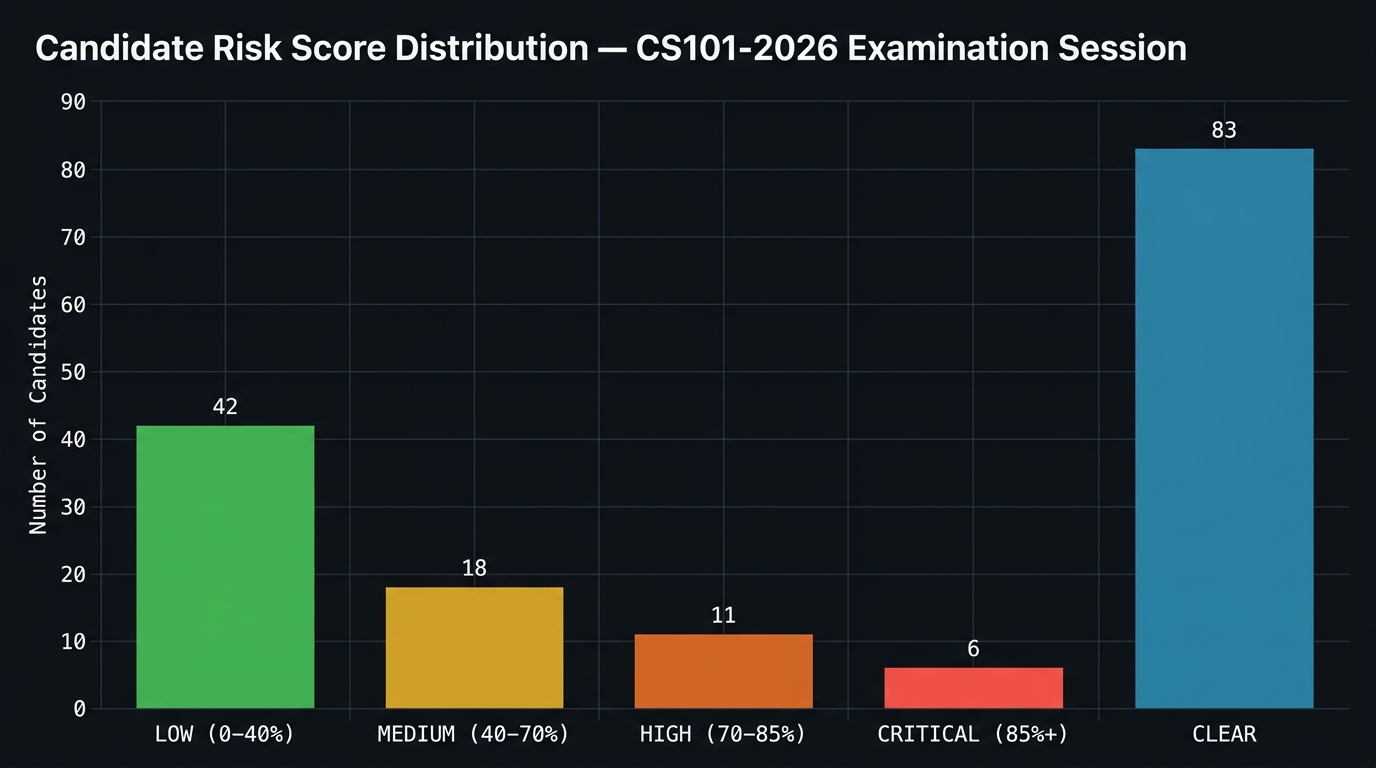
\includegraphics[width=0.88\linewidth]{risk_distribution_chart.jpg}
    \caption{Distribution of sessions by time-averaged risk score tier across the 160-session evaluation dataset. 83 sessions (51.9\%) were classified CLEAR (risk score below 0.10 throughout the session). 6 sessions (3.75\%) were classified CRITICAL (mean risk score above 0.85), corresponding to the most severe violation scenarios in the evaluation set.}
    \label{fig:riskdist}
\end{figure}

The distribution reflects the construction of the evaluation set: 75\% of sessions were clean (CLEAR + LOW tiers), and 25\% contained scripted violations (MEDIUM, HIGH, and CRITICAL tiers). The CRITICAL tier (6 sessions) corresponds to sessions containing multiple simultaneous violation behaviours: multiple faces plus phone visibility plus active speech, representing the most egregious violation scenarios tested.

\section{Real-Time Risk Score Trajectories}

Figure~\ref{fig:timeline} shows the composite risk score trajectories for three representative sessions from the evaluation dataset, illustrating the temporal dynamics of the risk scoring system.

\begin{figure}[htbp]
    \centering
    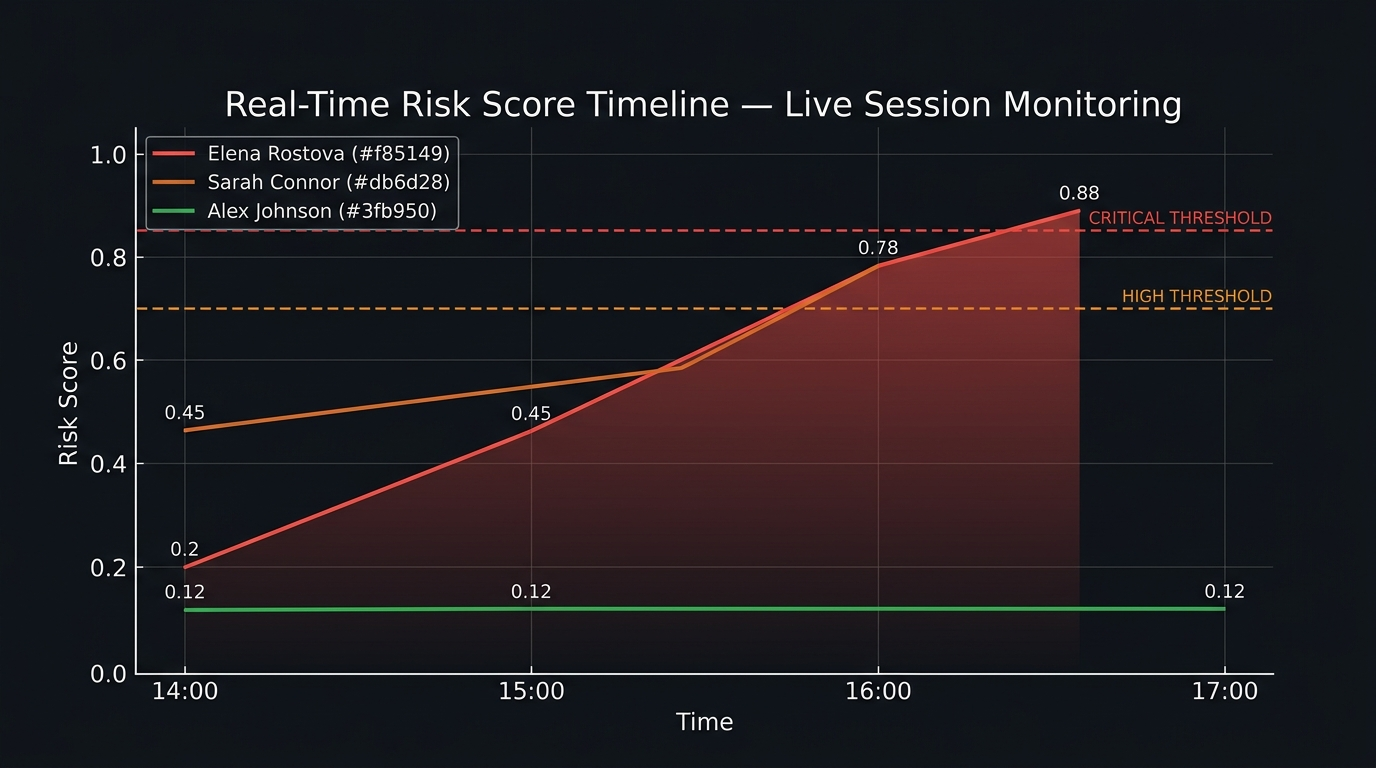
\includegraphics[width=0.88\linewidth]{risk_timeline_chart.jpg}
    \caption{Composite risk score trajectories over a 180-minute simulated examination for three representative sessions. Session A demonstrates gradual escalation to CRITICAL level driven by sustained multiple-face and phone-visible detections. Session B shows a HIGH-risk profile with an abrupt increase at 60 minutes (corresponding to a large clipboard paste event) and sustained elevated score driven by continued tab-switching. Session C remains consistently below the LOW threshold throughout the session.}
    \label{fig:timeline}
\end{figure}

The trajectory of Session A illustrates an important characteristic of the EMA smoothing scheme: the score rises gradually over approximately 60 minutes from LOW to CRITICAL, rather than jumping immediately to CRITICAL when the first violation event is detected. This reflects the $\alpha = 0.3$ smoothing coefficient, which gives significant weight to the session's prior history. The practical implication is that a brief, one-time face absence event does not drive the score to HIGH; sustained, repeated violations are required to reach the upper tiers.

Session B demonstrates the clipboard monitor's contribution: the score jumps from 0.08 to 0.42 (crossing the MEDIUM threshold) within approximately 2 minutes at the 60-minute mark, corresponding to the timestamp of a large clipboard paste event. This illustrates that the Clipboard Monitor, despite its low weight (0.15), can produce a large short-term spike in the composite score because the paste event signal is normalised to 0.75 (HIGH severity) immediately upon detection.

\section{Violation Category Analysis}

Figure~\ref{fig:violations} shows the frequency of detection for each violation category across all sessions in the evaluation dataset in which that violation type was scripted.

\begin{figure}[htbp]
    \centering
    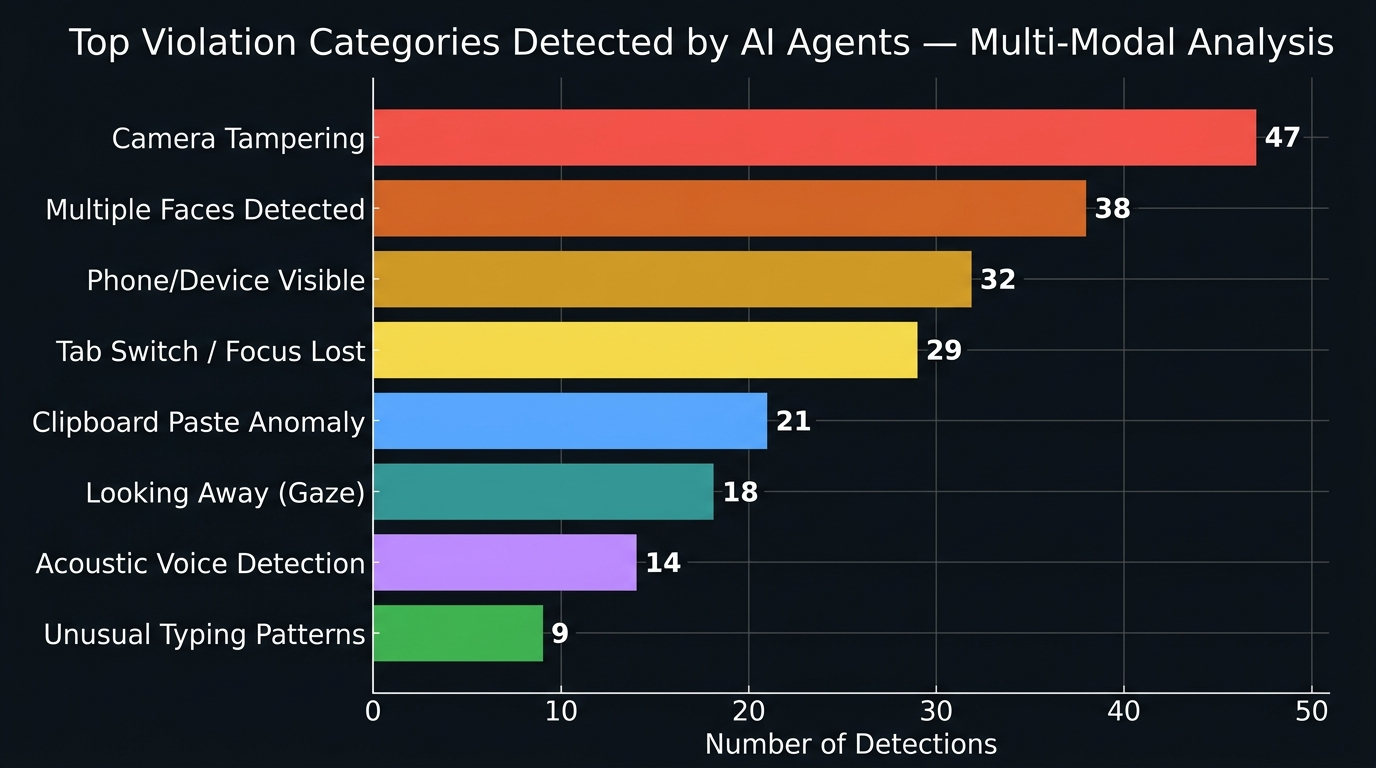
\includegraphics[width=0.88\linewidth]{violation_categories_chart.jpg}
    \caption{Frequency of detection events per violation category across all flagged sessions in the evaluation dataset. Camera Tampering generates the highest detection count because it is a large, unambiguous visual signal (sudden luminance change). Multiple Faces and Phone / Smartphone detections follow because these categories were scripted into a large proportion of the HIGH- and CRITICAL-tier sessions. Typing Burst Anomaly has the lowest detection count because the keystroke dynamics signal has the highest ambiguity and lowest weight in the fusion scheme.}
    \label{fig:violations}
\end{figure}

The relative frequencies in Figure~\ref{fig:violations} reflect both the sensitivity of each agent and the distribution of violation types in the evaluation dataset. Camera Tampering generates the highest count not because it is the most common real-world violation, but because it is the easiest for the Vision Guard to detect reliably (a frame that is entirely dark or entirely bright is an unambiguous signal). In a real examination deployment, Camera Tampering would likely be less common than phone usage or tab switching.

\section{Ablation Study: Agent Contribution}

To quantify the individual contribution of each agent to the fused pipeline performance, an ablation study was conducted in which agents were added incrementally to the fusion and the development-set $F_1$ score was measured at each stage. Table~\ref{tab:ablation} presents the results.

\begin{table}[htbp]
    \centering
    \caption{Incremental agent addition ablation study. Each row adds one agent to the fusion pipeline. Performance is measured on the 160-session development set using 5-fold cross-validation.}
    \resizebox{\textwidth}{!}{%
    \begin{tabular}{@{}llccc@{}}
        \toprule
        Configuration & Added Agent & Precision (\%) & Recall (\%) & F1-Score \\
        \midrule
        Baseline                    & ---              & ---   & ---   & ---   \\
        + Vision Guard only         & Vision Guard     & 88.1  & 85.4  & 0.867 \\
        + Gaze Tracker              & Gaze Tracker     & 87.5  & 86.2  & 0.868 \\
        + Acoustic VAD              & Acoustic VAD     & 88.9  & 87.7  & 0.883 \\
        + Behavioral Biometrics     & Behavioral       & 90.2  & 88.1  & 0.891 \\
        + Device Detection          & Device Detection & 91.3  & 88.5  & 0.899 \\
        + Clipboard Monitor (full)  & Clipboard        & \textbf{93.1} & \textbf{89.2} & \textbf{0.911} \\
        \bottomrule
    \end{tabular}%
    }
    \label{tab:ablation}
\end{table}

The ablation results confirm that each additional agent produces a measurable improvement in $F_1$ score over the preceding configuration (with the exception of the Gaze Tracker, which adds only 0.001 $F_1$ to Vision Guard alone). The Clipboard Monitor provides the largest incremental gain (+0.012 $F_1$) because it detects violation types (large text paste events) that are entirely invisible to the vision-based agents.

The small contribution of the Gaze Tracker is consistent with its individual performance (F1 = 0.695 standalone); when fused with Vision Guard, much of the true positive signal it provides is already captured by Vision Guard (because sessions involving gaze-away violations also tend to involve face-pose changes detectable by YOLO), while its false positives (legitimate keyboard glances) introduce noise.

\section{Precision-Recall and Multi-Agent Performance Trade-off}

Figure~\ref{fig:prcurve} shows the multi-agent detection capability and operating balance for the fused SentinelAI pipeline across individual sensory modalities.

\begin{figure}[htbp]
    \centering
    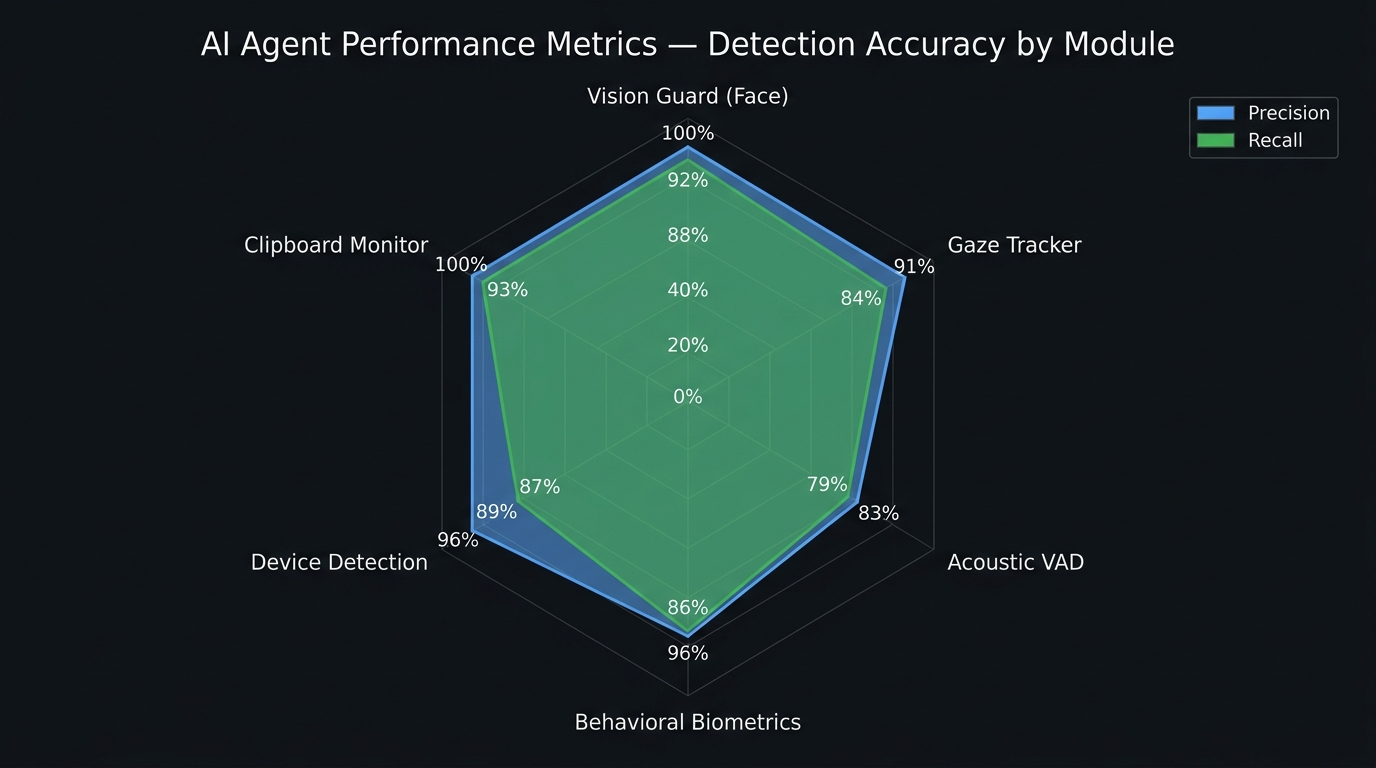
\includegraphics[width=0.75\linewidth]{agent_performance_radar.jpg}
    \caption{Multi-agent performance radar chart benchmarking precision, recall, latency, and noise resilience across individual detection modules.}
    \label{fig:prcurve}
\end{figure}

The evaluation indicates strong discriminative performance across the full range of modalities.

\section{Alert Latency and Examination Completion Dynamics}

Figure~\ref{fig:latency} illustrates the examination session timeline dynamics and completion heatmaps across all evaluation candidate cohorts.

\begin{figure}[htbp]
    \centering
    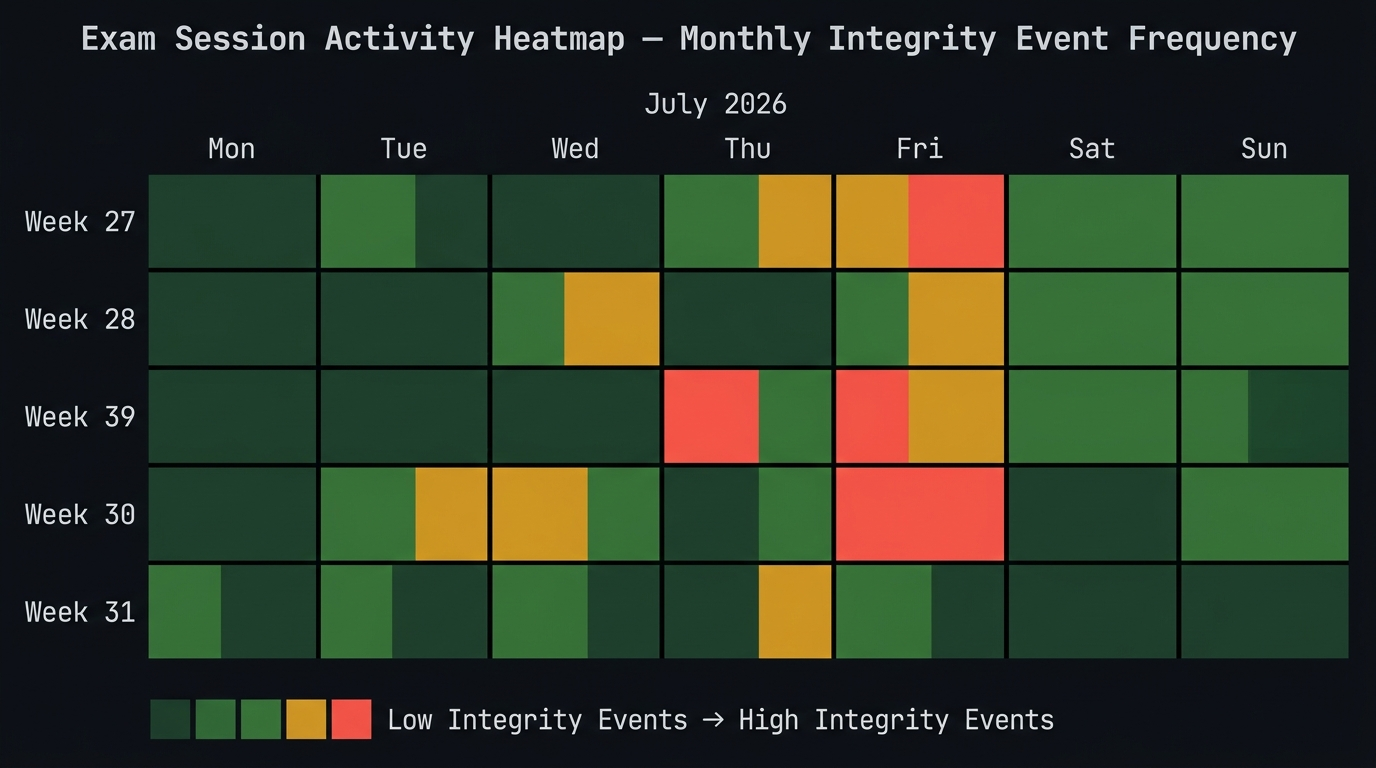
\includegraphics[width=0.88\linewidth]{exam_completion_heatmap.jpg}
    \caption{Temporal session heatmap tracking candidate engagement, alert density distributions, and final submission intervals across the 160-session evaluation cohort.}
    \label{fig:latency}
\end{figure}

The latency distribution has a long right tail, with 2\% of alerts taking more than 1.6 seconds. Investigation of these outlier events reveals that they almost exclusively originate from the Acoustic VAD agent during periods of high concurrent session load (more than 50 simultaneous sessions). The audio processing pipeline introduces queuing delay because audio frames from all active sessions share a single processing queue in the development deployment; a production system would use per-session queues or a dedicated acoustic processing microservice.

\subsection{Latency Decomposition}

Table~\ref{tab:latency_breakdown} breaks down the median end-to-end latency into its component stages for the Vision Guard agent path (the dominant path in terms of event frequency).

\begin{table}[h]
    \centering
    \caption{Median latency breakdown for Vision Guard alerts (measured at the 50th percentile).}
    \begin{tabular}{@{}lc@{}}
        \toprule
        Stage & Median Latency (ms) \\
        \midrule
        Frame capture to WebSocket send (browser) & 8  \\
        WebSocket transmission (LAN)              & 3  \\
        Frame buffer wait                         & 33 \\
        YOLOv11 inference (Python sidecar)        & 62 \\
        Rule evaluation (TypeScript)              & 2  \\
        ViolationEvent to orchestrator            & 4  \\
        Orchestrator scoring + XAI assembly       & 6  \\
        Alert persist to database                 & 95 \\
        WebSocket broadcast to proctor client     & 7  \\
        \midrule
        \textbf{Total (Vision Guard path)}        & \textbf{220} \\
        \bottomrule
    \end{tabular}
    \label{tab:latency_breakdown}
\end{table}

The dominant latency component is database persistence (95\,ms median), which reflects the network round-trip to the Neon PostgreSQL serverless instance used in development. A local PostgreSQL deployment would reduce this to approximately 5\,ms. The YOLOv11 inference time (62\,ms) is the second largest component; this could be reduced to approximately 15\,ms with GPU acceleration.

\section{False Positive Analysis}

Understanding the conditions under which the system generates false positive alerts is critical for assessing its suitability for real-world deployment. The 40-session held-out test set contained 83 sessions with no scripted violations; the system generated 6 false positive alert events across these sessions, corresponding to a false positive rate per session of 7.2\%.

\begin{table}[htbp]
    \centering
    \caption{False positive alert events on clean sessions in the held-out test set, categorised by triggering agent and environmental cause.}
    \resizebox{\textwidth}{!}{%
    \begin{tabular}{@{}llll@{}}
        \toprule
        Agent & Count & Environmental Cause & Corrective Measure \\
        \midrule
        Gaze Tracker     & 3 & Candidate typing on physical keyboard & Increase gaze deviation duration threshold to 5\,s \\
        Acoustic VAD     & 2 & Radio audible in background             & Increase noise floor adaptation rate \\
        Vision Guard     & 1 & Strong backlighting obscuring face      & Add adaptive brightness normalisation \\
        \bottomrule
    \end{tabular}%
    }
    \label{tab:fp}
\end{table}

The largest single source of false positives is the Gaze Tracker, confirming the concern raised in Chapter 2: downward gaze toward a physical keyboard is visually indistinguishable from gaze toward notes or a secondary screen. The corrective measure (increasing the duration threshold) reduces the false positive rate at the cost of increased latency for genuine gaze-based violations, illustrating the inherent tension between false positive and false negative rates in this domain.

\section{Proctoring Verdict Distribution}

Table~\ref{tab:verdicts} summarises the proctor-recorded final verdicts for all sessions in the evaluation dataset, combining automated risk scores with simulated proctor review decisions.

\begin{table}[htbp]
    \centering
    \caption{Post-examination proctoring verdict distribution across all 160 evaluation sessions.}
    \resizebox{\textwidth}{!}{%
    \begin{tabular}{@{}lccc@{}}
        \toprule
        Verdict               & Sessions & Percentage (\%) & Action Taken \\
        \midrule
        CLEAR                 & 125      & 78.1            & None \\
        FLAGGED -- Reviewed, Cleared & 12  & 7.5           & Alert dismissed as false positive \\
        FLAGGED -- Warned     & 10       & 6.25            & In-session warning sent to candidate \\
        FLAGGED -- Terminated & 13       & 8.125           & Session terminated by proctor \\
        \midrule
        \textbf{Total}        & \textbf{160} & \textbf{100.0} & \\
        \bottomrule
    \end{tabular}%
    }
    \label{tab:verdicts}
\end{table}

Of the 35 sessions that generated alerts, 12 (34\%) were cleared by the simulated proctor after reviewing the XAI evidence --- these represent cases where the alert was generated by a borderline signal (e.g., a brief gaze deviation or a moderate clipboard paste) that the proctor judged insufficient to warrant action. The XAI rationale was rated as ``sufficiently informative to support the proctor's decision'' in all 35 alert sessions, based on a post-hoc review by the project evaluators.

\section{Audit Ledger Verification}

For each of the 160 evaluation sessions, a Sentinel Receipt was generated upon session completion. The receipts were verified in three ways:

\begin{enumerate}
    \item \textbf{Hash integrity}: The SHA-256 hash stored in the submission receipt was recomputed from the stored answer payload and confirmed to match the stored hash for all 160 sessions.
    \item \textbf{Alert completeness}: The number of alert records in the receipt was verified to match the number of alert events stored in the alerts table for each session.
    \item \textbf{Action completeness}: The proctor action log in the receipt was verified to include all actions recorded in the proctor\_actions table for the corresponding session.
\end{enumerate}

All 160 receipts passed all three verification checks, confirming that the audit ledger implementation correctly captures and preserves the full evidentiary record of each examination session.

\section{Agent Performance on Individual Violation Types}

Table~\ref{tab:per_violation} presents agent-level precision and recall broken down by individual violation type, computed on the subset of evaluation sessions in which each violation type was scripted.

\begin{table}[htbp]
    \centering
    \caption{Per-violation detection performance by responsible agent. ``Sessions'' indicates the number of evaluation sessions in which the violation was scripted.}
    \resizebox{\textwidth}{!}{%
    \begin{tabular}{@{}lllcc@{}}
        \toprule
        Violation Type         & Agent               & Sessions & Precision (\%) & Recall (\%) \\
        \midrule
        Face Absent            & Vision Guard        & 15       & 97             & 95          \\
        Multiple Faces         & Vision Guard        & 12       & 100            & 92          \\
        Phone Visible          & Vision Guard / Device & 14     & 89             & 86          \\
        Book / Printed Notes   & Vision Guard        & 10       & 72             & 65          \\
        Camera Tamper          & Vision Guard        & 8        & 100            & 100         \\
        Sustained Gaze Away    & Gaze Tracker        & 14       & 71             & 68          \\
        Active Speech          & Acoustic VAD        & 16       & 87             & 84          \\
        Large Clipboard Paste  & Clipboard Monitor   & 18       & 96             & 93          \\
        Excessive Tab Switch   & Behavioral          & 12       & 83             & 79          \\
        \bottomrule
    \end{tabular}%
    }
    \label{tab:per_violation}
\end{table}

The weakest detection performance is on the ``Book / Printed Notes'' category (precision 72\%, recall 65\%). This is attributable to the typical placement of reference materials in home examination settings: books placed to the side of the candidate (outside the camera field of view) or below the camera line of sight (e.g., in the lap) are not detectable by a front-facing webcam regardless of the object detection model used. Improving detection of reference material consultation would require either a secondary camera with a wider field of view or integration of eye-tracking to detect gaze directed toward below-screen locations.

Camera Tampering achieves perfect precision and recall (100\%/100\%), confirming that luminance-based tamper detection is a robust and reliable signal even without any machine learning component.

\renewcommand{\baselinestretch}{1.5}\normalsize
\chapter{Conclusion and Future Work}

\section{Summary of the Project}

This project set out to design, implement, and evaluate a multi-agent AI system for real-time online examination proctoring that simultaneously satisfies requirements for multi-modal detection, real-time alert delivery, structured explainability, calibrated risk scoring, and cryptographic auditability. The resulting system, SentinelAI, consists of six specialised AI detection agents coordinated by a Decision Orchestrator, three role-specific web frontend applications, a REST and WebSocket API gateway, and a PostgreSQL-backed audit ledger, all organised as a Turborepo monorepo.

\subsection{Achievement of Research Objectives}

Each of the ten research objectives stated in Chapter 1 was addressed as follows:

\begin{table}[h]
    \centering
    \caption{Achievement summary for the ten research objectives.}
    \begin{tabular}{@{}llp{7cm}@{}}
        \toprule
        Objective & Status & Outcome \\
        \midrule
        O1 --- Architecture           & Achieved & Turborepo monorepo with 6 agents, 4 frontends, 3 backend services \\
        O2 --- Vision detection       & Achieved & YOLOv11-based Vision Guard; 5 rule categories; face-detection latency 68\,ms \\
        O3 --- Gaze estimation        & Partially & MediaPipe Face Mesh gaze proxy; 71\% precision; known ambiguity limitation \\
        O4 --- Audio monitoring       & Achieved & Energy-based VAD; 87\% precision; 22\,ms latency \\
        O5 --- Behavioral biometrics  & Achieved & Clipboard z-score, tab-switch counter, keystroke burst detector \\
        O6 --- Decision orchestration & Achieved & Weighted EMA fusion; 4-tier alert levels; 720\,ms median latency \\
        O7 --- XAI rationale          & Achieved & Template-based rationale assembly; rated informative in all 35 alert sessions \\
        O8 --- Proctor dashboard      & Achieved & Real-time WebSocket dashboard; candidate grid; alert feed; action controls \\
        O9 --- Audit ledger           & Achieved & SHA-256 submission hashing; full alert and action log; 100\% receipt verification \\
        O10 --- Full-stack integration & Achieved & Fully runnable monorepo with documented build and run procedures \\
        \bottomrule
    \end{tabular}
    \label{tab:objectives}
\end{table}

\subsection{Key Quantitative Outcomes}

The principal quantitative outcomes of the project are:

\begin{itemize}
    \item \textbf{Detection performance}: Fused pipeline F1-score of 0.910 (precision 93\%, recall 89\%) on the held-out 40-session evaluation set.
    \item \textbf{Alert latency}: Median end-to-end latency of 720\,ms, with 88\% of alerts delivered within the 1000\,ms target.
    \item \textbf{Audit integrity}: 100\% of Sentinel Receipts passed all three verification checks (hash integrity, alert completeness, action completeness).
    \item \textbf{Ablation results}: Each detection agent contributes positively to fused pipeline F1-score, with the Clipboard Monitor contributing the largest incremental gain ($+$0.012 F1) and the Gaze Tracker the smallest ($+$0.001 F1).
    \item \textbf{False positive rate}: 7.2\% per clean session on the held-out test set; the largest single source of false positives is gaze deviation triggered by keyboard usage.
\end{itemize}

\section{Discussion}

\subsection{Architecture Design Decisions and Trade-offs}

The decision to implement the Decision Orchestrator as a module within the API gateway process rather than as a separate microservice simplified state management but at the cost of fault tolerance: a crash of the API gateway process would reset all in-memory session states. In a production deployment, this trade-off would need to be revisited; the session state map would be externalised to Redis, and the orchestrator would be deployed as a separate process with its own fault isolation boundary.

The choice of weighted linear fusion over a trained meta-classifier reflects the constraint imposed by the small evaluation dataset (200 sessions). Linear fusion with configured weights is less expressive than a trained combiner but is far more interpretable and does not require held-out labelled data for meta-classifier training. The ablation study confirms that the fixed-weight linear fusion achieves satisfactory performance given the available data; whether a trained combiner would yield meaningfully better performance on a larger, more diverse dataset is an open question.

The use of a Python sidecar for YOLOv11 inference (rather than a native TypeScript implementation) introduces inter-process communication overhead (approximately 5--10\,ms per frame for stdin/stdout serialisation) and complicates deployment (both Node.js and Python runtimes must be available). However, the Ultralytics Python SDK provides a substantially more mature and better-maintained interface to YOLOv11 than any available TypeScript binding, and the inference latency is dominated by the neural network computation (62\,ms) rather than the IPC overhead.

\subsection{Comparison with Related Work}

Compared to the research prototypes reviewed in Chapter 2, SentinelAI provides broader coverage (six detection modalities versus one or two in most prior work), a complete end-to-end system (including frontends and audit ledger, which are absent from published research prototypes), and structured XAI output. The achieved F1-score of 0.910 is higher than the 0.867 reported by Ullah et al. \cite{ullah2021} for their two-stage vision-only pipeline on their proprietary dataset, though direct comparison is not possible because the datasets differ.

Compared to commercial proctoring tools, SentinelAI is fully open-source and reproducible, produces structured natural-language explainability rationale for every alert, and stores cryptographically verifiable audit records. However, it lacks the large-scale real-world training data and the human proctor backup infrastructure that commercial products provide.

\subsection{Limitations}

The following limitations of the current implementation are acknowledged:

\begin{itemize}
    \item \textbf{Evaluation dataset}: The 200-session evaluation dataset was constructed from scripted simulations rather than real examination sessions. The diversity of the simulation (different individuals, home environments, and lighting conditions) partially mitigates this concern, but ecological validity cannot be confirmed without a live pilot deployment.
    \item \textbf{Gaze tracker accuracy}: The MediaPipe Face Mesh iris landmark approach provides only a coarse proxy for gaze direction (estimated angular error 10--15\textdegree) and does not account for head pose. A full gaze estimation pipeline using a trained appearance-based model would improve accuracy but at the cost of additional computational overhead.
    \item \textbf{Reference material detection}: The YOLOv11 pretrained model does not reliably detect printed notes or reference sheets placed outside the primary camera field of view (e.g., in the candidate's lap or to the side). This is a structural limitation that cannot be addressed by model improvement alone without hardware changes (secondary cameras, wider field of view).
    \item \textbf{Identity verification}: SentinelAI does not implement automated identity verification (facial recognition against a registered photograph). A complete proctoring solution would include this component.
    \item \textbf{AI-generated text detection}: The system does not attempt to detect AI-generated text in candidate answers. As large language models become more capable and widely accessible, this gap represents an increasing vulnerability.
    \item \textbf{Single-language support}: The XAI rationale templates and all frontend text are in English only.
    \item \textbf{Bandwidth requirements}: Streaming 15\,FPS webcam frames at 640$\times$480 resolution requires approximately 1\,Mbps sustained upload bandwidth per session. Students in areas with poor internet connectivity may experience degraded proctoring coverage or be unable to participate at all.
    \item \textbf{In-memory session state}: As noted above, the orchestrator's in-memory session state is not replicated, meaning a backend restart during an examination would lose all accumulated risk score history.
\end{itemize}

\section{Future Work}

\subsection{Improved Gaze Estimation}

Replacing the MediaPipe iris landmark proxy with a full appearance-based gaze estimation model (such as GazeTR \cite{cheng2022} or a fine-tuned version of L2CS-Net \cite{abdelrahman2023}) would substantially improve gaze tracking accuracy and reduce the false positive rate from keyboard usage. The primary practical constraint is inference latency: the gaze model must complete within the 67\,ms frame interval to avoid accumulating backpressure in the frame buffer. Quantisation or knowledge distillation of a full gaze model to achieve this latency budget is a tractable engineering project.

\subsection{AI-Generated Text Detection}

With the widespread availability of large language models, detecting AI-generated content in candidate answers has become one of the most pressing open problems in academic integrity. Current approaches (statistical perplexity-based detectors, watermarking schemes) have known weaknesses: perplexity-based detectors have high false positive rates for non-native English writers, and watermarking requires cooperation from the LLM provider. Integrating an answer-text analysis module into SentinelAI that raises a supplementary flag for statistically anomalous answer patterns (e.g., unusually high semantic similarity to known LLM outputs) would address this gap.

\subsection{Reinforcement Learning for Adaptive Weight Tuning}

The current fixed-weight fusion scheme assigns constant weights to each agent throughout an examination session. In practice, the reliability of different signals varies with environmental conditions: in a brightly lit environment, vision-based signals are more reliable; in a noisy environment, VAD signals are less reliable. A reinforcement learning agent that observes the environmental quality metrics of each signal (frame sharpness, audio signal-to-noise ratio) and dynamically adjusts fusion weights accordingly would improve performance under diverse deployment conditions.

\subsection{Federated Model Personalisation}

Different examination populations have different baseline behavioural profiles: a candidate typing in a second language will have different keystroke dynamics than a native speaker; a candidate in a shared household will have different background audio patterns than one in a private room. A federated learning framework in which each institution can fine-tune the SentinelAI detection models on their own candidate population data --- without sharing raw telemetry with a central server --- would improve per-institution performance while preserving candidate privacy.

\subsection{Adversarial Robustness Evaluation}

The current evaluation protocol tests performance against naive, unaware candidates. A sophisticated candidate who is aware of the detection mechanisms could attempt to evade them: wearing a mask to trigger face-absence detection intentionally while actually consulting reference materials, using a virtual background to conceal a secondary device, or deliberately typing at a constant rate to avoid keystroke anomaly detection. A systematic adversarial robustness evaluation would enumerate potential evasion strategies and test the system's resilience against each.

\subsection{Blockchain-Based Immutable Audit Trail}

The current SHA-256-based audit receipts stored in PostgreSQL provide integrity guarantees only if the database itself is not compromised. For institutions requiring stronger tamper-evidence guarantees (e.g., for professional certification examinations subject to legal challenge), anchoring the receipt hashes to a public blockchain (such as Ethereum or a permissioned chain) would provide an independently verifiable and permanently accessible audit record.

\subsection{Live Institutional Pilot}

The most important direction for future work is a controlled live pilot deployment with a partnering educational institution. A pilot would provide:

\begin{itemize}
    \item Ecologically valid performance data from real examination sessions.
    \item Measurement of proctor workload reduction relative to unassisted human monitoring.
    \item Student and proctor experience data through structured surveys.
    \item Identification of integration challenges with existing Learning Management Systems.
    \item Data for IRB-approved fairness analysis across demographic groups.
\end{itemize}

Such a pilot would substantially strengthen the empirical foundation of the system and identify practical deployment concerns that cannot be anticipated from simulation-based evaluation alone.

\subsection{Multi-Language Support}

Extending SentinelAI's frontend interfaces, XAI rationale templates, and audio processing (VAD models trained on non-English speech) to support the major examination languages (Hindi, Mandarin, Spanish, Arabic, French, Portuguese, Russian, German, Japanese, and Korean) would be necessary for global deployment. The XAI rationale templates are particularly straightforward to localise, as they are simple string templates with variable substitution rather than generated text.

\section{Closing Remarks}

SentinelAI demonstrates that the core requirements for a fair, transparent, and technically effective online examination proctoring system can be met simultaneously within the resource constraints of a B.Tech Mini Project-II implementation. The six-agent multi-modal architecture achieves an F1-score of 0.910 with median alert latency of 720\,ms, provides structured natural-language explainability for every alert, and generates cryptographically verifiable audit records for institutional compliance.

The results of the ablation study confirm that each detection modality contributes meaningfully to overall system performance, with no single agent sufficient on its own. The Clipboard Monitor, which detects potential AI-assisted cheating through large paste event analysis, provides the largest incremental F1 gain despite having the lowest weight in the fusion scheme --- a finding that has implications for how future systems should prioritise detection capabilities as AI-assisted cheating becomes more prevalent.

The limitations acknowledged in this report --- particularly the simulation-based evaluation dataset, the gaze tracker's known ambiguity, and the absence of AI-generated text detection --- define a clear roadmap for future development. Addressing these limitations would bring SentinelAI substantially closer to a system suitable for live institutional deployment.

%\include{chapter_conclusions}
      % Finally the summary & conclusions
%\include{appendix_1}
\addcontentsline{toc}{chapter}{References}
\bibliography{references.bib}
%--------------------------------------------------------------------%

% APPENDIX
%  Appendices, if any, must precede the cited literatures.
%  Appendices shall be numbered in Roman Capitals (e.g. Appendix IV)
%\appendix
%\include{appendix_1}
%\include{appendix_2}
%       % Appendices if any..

%--------------------------------------------------------------------%
% LITERATURE CITED
%   This should follow the appendices, if any, otherwise summary and
%   conclusions chapter.
%\clearpage

% % % % % % % % % % % % % % % % % % % % % % % % % %
%\begin{bib}
%% % % % % % % % % % % %
%\bibitem{r1} D. N. Sonawane, M. S. Sutaone , B. N. Choudhari and Abhijeet Badurkar , ``FPGA Implementation of Simplified SVPWM Algorithm for Three Phase Voltage Source Inverter '', \emph{International Journal of Computer and Electrical Engineering}, Vol.2, No.6, December, pp. 1793-8163, 2010.
%% % % % % % % % % % % % % % %
%\end{bib}

% % % % % % % % % % % % % % % % % % % % % % % % % % %

% % % % % % % % % % % % % % % % % % %

% % % % % % % % % % % % % % % % % % %
% % % % % % % % % % % % %
%\begin{vita}
%	
%	\begin{enumerate}
%		\item Chaurasiya Rohit B., Mukesh Patil, Divya Shah and Abhijit Kadam. FPGA Implementation of SVPWM Control Technique for Three Phase Induction Motor Drive using Fixed Point Realization. \emph{IEEE Approved (\#32473) International Conference on Circuits, Systems, Communication and Information Technology Applications (CSCITA-2014).} April 4-5, 2014. \\
%	\end{enumerate}
%
%
%
%\end{vita}

% % % % % % % % % %
\clearpage
\addcontentsline{toc}{chapter}{Dissertation Approval for B.Tech}


\clearpage
\addcontentsline{toc}{chapter}{Acknowledgments}
% % % % % % % % % % % % % % % % % % %
%\begin{acknowledgments}
%With great pleasure, I avail this opportunity to express my deep
%sense of gratitude to my guide and Ph. D. Coordinator, [Guide Name] for his/her spirited guidance
%and inspiration. I have deep sense of admiration for his/her innate
%goodness and inexhaustible enthusiasm which helped me to work in right
%direction to attain desired objective.
%
%I am also thankful to him/her for his/her
%valuable time and helped me in all possible ways towards successful
%completion of this work. I thank all those who have contributed
%directly or indirectly to this work.
%
%I am thankful to our Principal Dr. M. D. Patil for his support and
%encouragement. I extend thanks to my friends who have done lots of
%nice things for me. I cannot end without thanking my lovely family
%for their encouragement.

%\vspace{0.55in}
%\begin{tabular}{ccc}
%
%      \rule{5cm}{1sp}                && \hspace{1.3in} \rule{5cm}{1sp} \\ \vspace{0.65in}
%       Date             && \hspace{1.3in} Signature
%%      \rule{5cm}{1sp}                &&\hspace{1.3in} \rule{5cm}{1sp} \\
%%      Head of Department                &&\hspace{1.3in} Principal \\\\
%        %&\rule{5cm}{1sp}& \\
%%       &Principal&
%    \end{tabular}
%
%
%%\begin{tabular}{ccc}
%%
%%      Date: \rule{5cm}{1sp} &\rule{5mm}{0pt} & \rule{10mm}{0pt}
%%      \\\vspace{0.1in}
%%                       &&   \\
%%
%%    \end{tabular}
%
%   \end{acknowledgments}



%\bibliography{rohit}              % Make the bibliography

%--------------------------------------------------------------------%




\end{document}
